\documentclass[11pt,a4paper]{article}

\usepackage{kotex}
\usepackage{amsmath,amssymb,amsthm,mathtools,bm}
\usepackage{booktabs,tabularx,longtable,array}
\usepackage{graphicx}
\usepackage{caption}
\usepackage{subcaption}
\usepackage{geometry}
\usepackage{enumitem}
\usepackage{xcolor}
\usepackage{hyperref}
\usepackage{listings}
\usepackage{float}
\usepackage{tcolorbox}
\tcbuselibrary{breakable,skins}

\geometry{margin=25mm}
\graphicspath{{report_figures/}}
\hypersetup{
  colorlinks=true,
  linkcolor=blue!60!black,
  citecolor=blue!60!black,
  urlcolor=blue!60!black
}
\setlist[itemize]{leftmargin=2em}
\setlist[enumerate]{leftmargin=2em}
\lstset{
  basicstyle=\ttfamily\small,
  breaklines=true,
  frame=single,
  columns=fullflexible
}
\sloppy

% ---- 섹션 번호: 최상위 로마 숫자, 하위 알파벳 ----
\renewcommand{\thesection}{\Roman{section}}
\renewcommand{\thesubsection}{\Alph{subsection}}

% ---- 캡션 형식: 그림은 "Fig N.", 표는 "표 N" ----
\captionsetup[figure]{name=Fig,labelsep=period}
\captionsetup[table]{name=표,labelsep=space}
\captionsetup[sub]{labelformat=parens}

% ---- 수학 매크로 ----
\newcommand{\E}{\mathcal{E}}
\newcommand{\N}{\mathcal{N}}
\newcommand{\Hcal}{\mathcal{H}}
\newcommand{\Tr}{\operatorname{Tr}}
\newcommand{\Choi}{C_{\mathcal{E}}}
\newcommand{\id}{\mathrm{id}}
\newcommand{\Pos}{\mathrm{Pos}}
\newcommand{\Dens}{\mathrm{D}}
\newcommand{\Lin}{\mathrm{L}}
\newcommand{\diamondnorm}[1]{\left\lVert #1 \right\rVert_{\diamond}}
\newcommand{\onenorm}[1]{\left\lVert #1 \right\rVert_{1}}
\newcommand{\rank}{\operatorname{rank}}
\newcommand{\vecop}{\operatorname{vec}}
\DeclareMathOperator{\sgn}{sgn}

% ---- 정리 환경 ----
\theoremstyle{definition}
\newtheorem{definition}{정의}[section]
\newtheorem{example}{예제}[section]
\theoremstyle{plain}
\newtheorem{theorem}{정리}[section]
\newtheorem{proposition}{명제}[section]
\newtheorem{property}{성질}[section]
\newtheorem{corollary}{따름정리}[section]
\theoremstyle{remark}
\newtheorem*{remark}{참고}

% ---- 색상 상자 ----
\newtcolorbox{conceptbox}[1]{
  colback=blue!4!white, colframe=blue!50!black,
  fonttitle=\bfseries, title={#1},
  breakable, boxrule=0.6pt, arc=2pt}
\newtcolorbox{intuitionbox}{
  colback=green!4!white, colframe=green!45!black,
  breakable, boxrule=0.6pt, arc=2pt,
  left=4pt,right=4pt,top=3pt,bottom=3pt}
\newtcolorbox{mathbox}[1]{
  colback=orange!4!white, colframe=orange!55!black,
  fonttitle=\bfseries, title={#1},
  breakable, boxrule=0.6pt, arc=2pt}

\title{\textbf{양자 채널의 Choi 표현을 이용한 채널 분석과 응용\\[5pt]
\large{--- 직관과 수식을 함께 정리한 보고서 ---}}}
\author{이름 : 이재현 (2025-18876)}
\date{\today}

\begin{document}
\maketitle

\begin{abstract}
본 보고서는 같은 프로젝트에서 작성한 두 판본, 즉 직관을 중심으로 한 ``초심자용 안내서''와 수식을 중심으로 한 ``이론 해설본''을 하나로 합쳐 정리한 것이다. 이때 이해를 돕기 위한 내용(읽기 경로, 손계산 예제, 요약 치트시트, 용어집)도 함께 보강했다. 본 보고서의 목표는 ``quantum channel을 \textbf{Choi matrix}라는 하나의 행렬로 바꾸면, 서로 달라 보이는 다섯 가지 주제가 모두 같은 언어로 연결된다''는 점을, 왜 그런지에 대한 직관과 검증 가능한 등식 및 정리로 동시에 확인하는 것이라고 할 수 있다.

이를 위해 본문은 모든 핵심 개념을 (i)~말로 된 직관, (ii)~번호를 붙인 정의/성질/정리, (iii)~한 줄 수식 요약의 세 겹으로 설명했다. 양자역학의 가장 기초(상태, 측정, superposition)만 아는 독자를 위해 density matrix, tensor product, partial trace, quantum channel, complete positivity(CP), trace preservation(TP), Bloch sphere를 먼저 정의한 뒤, channel의 세 가지 동치 표현(Kraus, Stinespring, Choi)과 이들을 잇는 \textbf{Choi--Jamio{\l}kowski isomorphism}
\[
\E\text{ CP}\iff C_\E\succeq0,\qquad \E\text{ TP}\iff \Tr_B(C_\E)=I_A
\]
을 증명 개요와 함께 제시했다. 그 위에서 다섯 작업, 즉 표현 변환 검증, process tomography, diamond norm 기반 channel discrimination, quantum comb를 이용한 non-Markovian 분석, interactive 시각화를 각각 fidelity 관계식 $F_{\mathrm{avg}}=\frac{dF_{\mathrm{pro}}+1}{d+1}$, Helstrom 한계, Watrous SDP, BLP/RHP measure, link product 같은 정량적 도구와 함께 전개했다. 모든 그림과 표, 수치는 원본과 동일하게 유지하되, 각 수치가 어떤 식에서 나오는지를 함께 명시했다.
\end{abstract}

\tableofcontents
\newpage

%==================================================================
\section{이 보고서를 읽는 방법}
%==================================================================

본 보고서는 한 권 안에서 직관과 수식을 모두 다룬다. 이에 따라 독자의 배경에 맞추어 두 가지 읽기 경로를 활용할 수 있다.

\begin{itemize}
  \item \textbf{직관 트랙(처음 접하는 독자):} 각 절의 파란 \emph{개념 상자}와 초록 \emph{직관 요약}을 먼저 따라 읽고, 정리와 증명은 건너뛴다. 이때 그림과 표의 해석 문단을 함께 읽으면 큰 줄기를 잡을 수 있었다.
  \item \textbf{수식 트랙(이론을 확인하려는 독자):} 번호를 붙인 \emph{정의/성질/정리}와 주황 \emph{수식 상자}를 중심으로 읽는다. 이때 각 수치 결과에는 그 값을 낳는 식이나 정리 번호가 달려 있다.
\end{itemize}

\begin{conceptbox}{세 가지 상자의 역할}
\begin{description}[leftmargin=1.4em,style=nextline]
  \item[\textcolor{blue!60!black}{$\blacksquare$} 개념 상자 (파랑)] 새 용어를 도입하고 그 의미를 설명한다.
  \item[\textcolor{green!50!black}{$\blacksquare$} 직관 요약 (초록)] ``결국 한 문장으로 무슨 뜻인가''를 정리한다.
  \item[\textcolor{orange!70!black}{$\blacksquare$} 수식 상자 (주황)] 정의식, 핵심 성질, 수치 재현을 모은다.
\end{description}
더불어 정의 / 성질 / 명제 / 정리 / 예제는 번호를 붙인 환경으로 제시하여 추적할 수 있도록 했다.
\end{conceptbox}

\begin{conceptbox}{표기 약속(notation)}
\begin{itemize}[leftmargin=1.4em]
  \item $\Hcal_A,\Hcal_B$: 유한 차원 복소 Hilbert space, $d_A=\dim\Hcal_A$. qubit은 $d=2$.
  \item $\Lin(\Hcal)$: $\Hcal$ 위 linear operator 전체. $\Pos(\Hcal)=\{X\succeq0\}$, $\Dens(\Hcal)=\{\rho\succeq0,\Tr\rho=1\}$.
  \item $X^\dagger$ conjugate transpose, $X^T$ transpose, $\overline{X}$ 성분별 켤레복소.
  \item $\succeq0$: positive semidefinite(모든 eigenvalue $\ge0$). $\onenorm{X}=\Tr\sqrt{X^\dagger X}$: trace norm.
  \item $I_A$ identity operator, $\{|i\rangle\}$ computational basis, Pauli $X,Y,Z$, $\vec\sigma=(X,Y,Z)$.
\end{itemize}
\end{conceptbox}

마지막에 Appendix로 ``개념 $\to$ 직관 $\to$ 핵심 식''을 한 장에 모은 요약 치트시트와, 영문 용어집을 함께 두었다. 급할 때는 치트시트만 보아도 전체 지도를 얻을 수 있을것으로 생각된다.

%==================================================================
\section{준비: 본론을 읽기 위한 도구들}
%==================================================================

이 장의 목표는 하나다. 뒤에서 ``channel을 Choi matrix로 바꾼다''는 문장이 나왔을 때, 그 한 문장의 모든 단어가 이미 친숙해지도록 만드는 것이라고 할 수 있다. 이에 각 도구를 직관과 수식으로 동시에 정의했다.

\subsection{양자 상태: 상태벡터에서 density matrix로}

기초 양자역학에서 한 양자계의 상태는 상태벡터 $|\psi\rangle$로 적는다. qubit은 $|\psi\rangle=\alpha|0\rangle+\beta|1\rangle$, $|\alpha|^2+|\beta|^2=1$처럼 두 basis 상태의 superposition으로 나타난다. 이렇게 단 하나의 벡터로 완전히 적히는 상태를 \textbf{pure state}라 한다. 그러나 실제로는 ``70\%로 $|0\rangle$, 30\%로 $|1\rangle$''처럼 고전적 확률이 섞인 \textbf{mixed state}가 흔하고, 이는 하나의 벡터로 적을 수 없다. 이에 \textbf{density matrix} $\rho$를 도입했다.

\begin{conceptbox}{개념: density matrix $\rho$}
pure state는 $\rho=|\psi\rangle\langle\psi|$, mixed state는 확률 $p_k$로 $\rho=\sum_k p_k|\psi_k\rangle\langle\psi_k|$로 적는다. 직관적으로 상태에 대해 알고 있는 모든 통계를 담은 행렬이라고 생각할 수 있다.
\end{conceptbox}

\begin{definition}[density matrix]
계 $\Hcal$의 상태는 $\rho=\rho^\dagger,\ \rho\succeq0,\ \Tr\rho=1$을 만족하는 operator $\rho\in\Lin(\Hcal)$이다.
\end{definition}

\begin{property}[density matrix의 기본 성질]\label{prop:density}
임의의 density matrix $\rho$에 대하여 다음이 성립한다.
\begin{enumerate}[label=\textup{(\roman*)}]
  \item \textbf{spectral decomposition} $\rho=\sum_i\lambda_i|e_i\rangle\langle e_i|$, $\lambda_i\ge0,\ \sum_i\lambda_i=1$ (eigenvalue들이 확률분포를 이룬다).
  \item \textbf{expectation value} $\langle A\rangle=\Tr(\rho A)$.
  \item \textbf{purity} $\Tr(\rho^2)=\sum_i\lambda_i^2\le1$, 등호 $\iff$ pure state.
\end{enumerate}
\end{property}
\begin{proof}[증명 개요]
(i)~Hermitian이고 $\succeq0$이므로 spectral theorem으로 $\lambda_i\ge0$, $\sum_i\lambda_i=\Tr\rho=1$로 계산된다. (ii)~$\Tr$의 선형성과 순환성으로 성립한다. (iii)~$\sum\lambda_i=1,\lambda_i\ge0$이면 $\sum\lambda_i^2\le(\sum\lambda_i)^2=1$이고, 등호는 rank-1일 때라고 할 수 있다.
\end{proof}

\begin{intuitionbox}
\textbf{직관:} 성질 \ref{prop:density}의 ``eigenvalue가 음이 아니다''와 정의의 ``trace가 1이다''라는 두 조건이 이 보고서 전체의 씨앗이 된다. channel의 물리성 조건(CP/TP)이 바로 이 둘을 일반화한 것이라고 할 수 있었다.
\end{intuitionbox}

\subsection{trace와 partial trace}

\begin{conceptbox}{개념: trace와 partial trace}
\textbf{trace} $\Tr(M)$은 대각 성분의 합으로, $\Tr(\rho)$는 ``전체 확률'', $\Tr(\rho A)$는 ``$A$의 expectation value''에 대응한다. \textbf{partial trace}는 joint state에서 한 계를 측정하지 않고 무시했을 때 남는 상태를 준다.
\end{conceptbox}

\begin{definition}[partial trace]
$\Tr_B:\Lin(\Hcal_A\otimes\Hcal_B)\to\Lin(\Hcal_A)$,
\[
\Tr_B(M)=\sum_k(I_A\otimes\langle k|_B)\,M\,(I_A\otimes|k\rangle_B),
\]
이때 $\{|k\rangle_B\}$는 임의의 orthonormal basis이며, 정의는 basis 선택과 무관하다.
\end{definition}

\begin{property}[partial trace의 성질]\label{prop:ptrace}
$\Tr_B$는 선형이고 $\Tr_A\circ\Tr_B=\Tr$, $\Tr_B(\rho_A\otimes\rho_B)=\rho_A\Tr(\rho_B)$, 더불어 $M\succeq0\Rightarrow\Tr_B(M)\succeq0$이다. reduced state는 $\rho_A=\Tr_B(\rho_{AB})$로 주어진다.
\end{property}

\subsection{두 계를 합치기: tensor product와 entanglement}

qubit 여럿을 함께 다루려면 \textbf{tensor product} $\otimes$가 필요하다. 차원 $d_A,d_B$의 두 계를 합치면 joint 계는 차원 $d_Ad_B$가 된다(qubit 둘이면 $4$, basis는 $|00\rangle,|01\rangle,|10\rangle,|11\rangle$).

\begin{conceptbox}{개념: entanglement}
joint state가 항상 $\rho_A\otimes\rho_B$처럼 두 부분의 곱으로 쪼개지지는 않는다. 쪼개지지 않는 상태가 \textbf{entangled} 상태이다. 뒤에서 ``보이지 않는 reference system과의 entanglement''이 complete positivity(CP)와 channel 구별 성능의 열쇠가 된다.
\end{conceptbox}

\begin{definition}[maximally entangled state]
$\Hcal_A\cong\Hcal_B\cong\mathbb C^d$에서 비정규화 $|\Omega\rangle=\sum_{i=1}^d|i\rangle_A|i\rangle_B$ ($\langle\Omega|\Omega\rangle=d$), 정규화 $|\Phi\rangle=\tfrac1{\sqrt d}|\Omega\rangle$로 둔다. qubit에서 $|\Phi\rangle=\tfrac1{\sqrt2}(|00\rangle+|11\rangle)$이다.
\end{definition}

\begin{property}[ricochet/transpose 항등식]\label{prop:ricochet}
임의의 $M$에 대해 $(M\otimes I)|\Omega\rangle=(I\otimes M^T)|\Omega\rangle$이 성립한다.
\end{property}
\begin{proof}
$(M\otimes I)|\Omega\rangle=\sum_{ij}M_{ji}|j\rangle|i\rangle$, $(I\otimes M^T)|\Omega\rangle=\sum_{ij}M_{ij}|i\rangle|j\rangle$이다. 이때 더미 지표 $i\leftrightarrow j$를 교환하면 두 식이 같음을 알 수 있었다.
\end{proof}

성질 \ref{prop:ricochet}은 Choi matrix에서 channel action을 복원하는 공식(정리 \ref{thm:recover})과, 뒤의 SDP 파트에서 ``entanglement이 정보를 더한다''는 사실을 떠받친다.

\subsection{quantum channel: unitary만으로 부족한 이유}

닫힌 계의 변화는 unitary $U$로 $\rho\mapsto U\rho U^\dagger$이다(noise가 없는 이상적 경우). 그러나 실제 장치에서는 qubit이 environment와 상호작용해 에너지가 새는 \textbf{relaxation}, 위상이 흐트러지는 \textbf{dephasing}, 그리고 calibration error가 함께 일어난다. 이렇게 열린 계의 변화는 unitary 하나로 적을 수 없고, 더 일반적인 \textbf{quantum channel}이 필요하다.

\begin{conceptbox}{개념: quantum channel $\E$와 CP/TP}
quantum channel은 density matrix를 density matrix로 보내는 linear map이다. 물리적이려면 \textbf{TP}(전체 확률 보존)와 \textbf{CP}(보이지 않게 entangled된 계까지 고려해도 결과가 정상)를 만족해야 한다.
\end{conceptbox}

\begin{definition}[quantum channel]
linear map $\E:\Lin(\Hcal_A)\to\Lin(\Hcal_B)$가 다음을 만족하면 channel(CPTP map)이다.
\begin{itemize}[leftmargin=1.6em]
  \item \textbf{TP:} 모든 $X$에 대해 $\Tr[\E(X)]=\Tr[X]$.
  \item \textbf{CP:} 모든 $n$에 대해 $\E\otimes\id_n$이 positivity를 보존, 즉 $X\succeq0\Rightarrow(\E\otimes\id_n)(X)\succeq0$.
\end{itemize}
\end{definition}

\begin{mathbox}{왜 ``positive''가 아니라 ``completely positive''인가}
$n=1$의 positivity만으로는 부족하다. 반례는 transpose map $T(\rho)=\rho^T$로, $T$는 positive이지만 completely positive는 아니다:
\[
(T\otimes\id)(|\Phi\rangle\langle\Phi|)=\tfrac12\,\mathrm{SWAP}\quad\text{는 eigenvalue }-\tfrac12\text{ 을 가진다.}
\]
즉 남몰래 entangled된 reference system까지 고려하면 $T$는 비물리적이다. CP는 ``임의의 reference system 확장에서도 정당함''을 요구한다고 할 수 있다.
\end{mathbox}

\begin{intuitionbox}
\textbf{직관:} TP는 ``확률이 새지 않는다'', CP는 ``남몰래 entangled된 계까지 고려해도 결과가 정상이다''이다. 물리적 channel $=$ TP $+$ CP라고 정리할 수 있다. 이 추상적 조건을 계산 가능하게 만드는 것이 다음 장의 Choi matrix이다.
\end{intuitionbox}

\subsection{한 qubit을 보는 그림: Bloch sphere}

\begin{conceptbox}{개념: Bloch sphere}
qubit 상태는 $\rho=\tfrac12(I+\vec r\cdot\vec\sigma)$, $\vec r=(r_x,r_y,r_z)$로 단위 구 위 또는 안의 점이 된다. 표면($|\vec r|=1$)은 pure, 내부는 mixed, 중심($\vec r=0$)은 maximally mixed state $I/2$에 대응한다. channel은 구를 affine 변환 $\vec r\mapsto M\vec r+\vec t$로 찌그러뜨리고($M$) 중심을 옮긴다($\vec t$).
\end{conceptbox}

\begin{property}[Bloch sphere와 PSD]
$\rho=\tfrac12(I+\vec r\cdot\vec\sigma)$의 eigenvalue는 $\tfrac{1\pm|\vec r|}{2}$이고, purity는 $\Tr(\rho^2)=\tfrac{1+|\vec r|^2}{2}$이다. 이에 따라 $\rho\succeq0\iff|\vec r|\le1$임을 알 수 있다.
\end{property}

\begin{conceptbox}{개념: unital channel}
$\E(I)=I$이면 \textbf{unital}, 즉 maximally mixed state($I/2$, 구의 중심)를 보존한다($\vec t=0$). 이때 주의할 점은 unital과 TP가 다른 조건이라는 것이다. TP는 ``전체 확률 보존(출력 측)'', unital은 ``중심 고정(입력 측)''을 의미한다. amplitude damping은 TP이지만 unital이 아니다.
\end{conceptbox}

\begin{itemize}
  \item \textbf{depolarizing noise}: 구를 모든 방향으로 균일하게 수축시키며($\vec t\approx0$) 중심을 유지한다.
  \item \textbf{amplitude damping noise}: excited state가 ground state로 내려가 구를 줄이면서 중심을 이동시킨다($\vec t\neq0$). 이는 비-unital이다.
\end{itemize}

이를 통해 본론에 필요한 도구가 모두 준비되었다고 할 수 있다: density matrix, tensor product와 entanglement, partial trace, quantum channel, CP/TP, Bloch sphere.

%==================================================================
\section{서론: 왜 Choi matrix인가}
%==================================================================

모든 linear map이 물리적 channel은 아니다. channel은 TP여야 하고, reference system과의 entanglement까지 고려한 CP여야 한다. 이 조건 중 reference system을 아무리 크게 붙여도 정당해야 한다는 CP는 처음에는 다루기 까다롭다. 이때 \textbf{Choi matrix를 쓰면 이 조건이 단순해진다}. CP는 어떤 행렬의 eigenvalue가 음이 아니라는 조건으로, TP는 어떤 partial trace가 identity가 된다는 조건으로 내려온다.

\begin{conceptbox}{개념: Choi matrix (이 보고서의 주인공)}
입력 계 $A$와 똑같은 짝을 하나 더 준비해 maximally entangled state를 만든 뒤, 한쪽에만 channel $\E$를 통과시킨다. 그 결과 남는 joint state가 Choi matrix이다. 즉 channel 전체를 사진 한 장으로 찍은 것이라고 생각할 수 있다.
\end{conceptbox}

\subsection{Choi matrix란 정확히 무엇인가 --- 세 가지 그림}

위 한 문장만으로는 Choi matrix가 구체적으로 어떤 행렬인지 잘 와닿지 않는다. 이에 같은 대상을 세 가지 그림으로 나누어 보았다. 세 그림은 모두 같은 행렬을 가리키며, 이 한 행렬이 어떻게 channel 전체를 담는지, 그리고 왜 CP가 eigenvalue 조건이 되는지를 각각 다른 각도에서 설명한다.

\paragraph{그림 1 --- channel의 응답표 (block matrix).}
quantum channel $\E$는 linear하다. 이에 임의의 입력 $\rho$를 basis 성분으로 펼치면
\[
\rho=\sum_{i,j}\rho_{ij}\,|i\rangle\langle j|
\quad\Longrightarrow\quad
\E(\rho)=\sum_{i,j}\rho_{ij}\,\E(|i\rangle\langle j|)
\]
이 된다. 즉 \textbf{channel이 각 기본 block $|i\rangle\langle j|$에 무엇을 하는지($\E(|i\rangle\langle j|)$)만 알면, 임의의 입력에 대한 답을 전부 알 수 있었다.} Choi matrix는 바로 이 응답들을 한 곳에 모아 둔 표이다. $(i,j)$ 칸에 $\E(|i\rangle\langle j|)$를 넣은 block matrix로 나타낼 수 있다:
\[
C_\E=
\begin{pmatrix}
\E(|0\rangle\langle 0|) & \E(|0\rangle\langle 1|) & \cdots\\
\E(|1\rangle\langle 0|) & \E(|1\rangle\langle 1|) & \cdots\\
\vdots & & \ddots
\end{pmatrix}.
\]
qubit($d=2$)이라면 $2\times2$ 칸 각각이 $2\times2$ block이므로 전체는 $4\times4$ 행렬이 된다. 이 그림에서 Choi matrix는 channel의 응답을 한 표에 모아 둔 lookup table에 해당한다.

\begin{intuitionbox}
\textbf{직관:} channel이 linear하기 때문에, 모든 입력에 대한 답이 기본 block $d^2$개에 대한 답으로 압축된다. Choi matrix는 그 $d^2$개의 답을 한 행렬에 정리한 것이다. 이를 통해 하나의 행렬이 channel 전체와 동등해진다(정리 \ref{thm:recover}이 이 복원을 식으로 보장한다).
\end{intuitionbox}

\paragraph{그림 2 --- entangled 쌍의 절반을 통과시키기(실험 레시피).}
그림 1에는 함정이 하나 있다. $|0\rangle\langle0|,|1\rangle\langle1|$은 실제 상태(density matrix)이지만, $|0\rangle\langle1|$ 같은 비대각 block은 그 자체로는 물리적 상태가 아니다($\Tr=0$, 음의 eigenvalue). 이에 $|0\rangle\langle1|$을 channel에 직접 넣어 볼 수는 없다. 그렇다면 응답 $\E(|0\rangle\langle1|)$는 어떻게 물리적으로 얻을 수 있는가. 이때 entanglement을 쓰면 된다.

\begin{conceptbox}{Choi matrix를 만드는 실험 레시피}
\begin{enumerate}[leftmargin=1.6em]
  \item 똑같은 두 계 $A,B$를 maximally entangled state $|\Phi\rangle=\tfrac1{\sqrt d}\sum_i|i\rangle_A|i\rangle_B$로 준비한다.
  \item 계 $A$는 건드리지 않고 그대로 둔다. 계 $B$만 channel $\E$에 통과시킨다.
  \item 남은 두 계의 joint state를 tomography로 측정한다. 이때 그 상태가 정규화된 Choi matrix $\rho_\E=C_\E/d$이다.
\end{enumerate}
\end{conceptbox}

왜 이 한 번의 실험이 channel 전체를 담는가. maximally entangled state에는 모든 basis 입력이 correlation 형태로 동시에 들어 있어서, $B$에만 channel을 걸어도 $A$와의 correlation에 비대각 응답 $\E(|i\rangle\langle j|)$까지 전부 기록되기 때문이라고 생각된다(이를 보장하는 것이 성질 \ref{prop:ricochet}의 transpose 항등식이다). 직접 넣을 수 없던 $|i\rangle\langle j|$의 응답을, entanglement을 통해 간접적으로 한꺼번에 읽어낼 수 있었다.

\begin{intuitionbox}
\textbf{직관:} channel을 검사할 때 입력을 하나씩 넣는 대신, 완벽히 correlated된 기준 신호인 entangled 쌍의 절반을 통과시킨다. channel이 남긴 흔적이 쌍의 correlation에 그대로 새겨져, 단 한 번의 측정으로 channel의 모든 응답을 잡아낼 수 있었다.
\end{intuitionbox}

\paragraph{그림 3 --- Choi matrix는 사실 진짜 양자 상태다 ($\Rightarrow$ 왜 CP $\iff$ eigenvalue $\ge0$).}
그림 2의 레시피에서 마지막에 손에 쥐는 것은 실제 실험으로 만들어 낸 두 계의 joint state이다. channel $\E$가 물리적(CP)이라면, 그 출력은 당연히 정당한 양자 상태여야 한다. 즉 Hermitian이고, eigenvalue가 음이 아니며($\succeq0$), 정규화하면 trace가 $1$이다. \textbf{이것이 $\E$ CP $\iff C_\E\succeq0$의 직관적 정체라고 할 수 있다.}

거꾸로 어떤 map이 만든 Choi matrix에 음의 eigenvalue가 하나라도 있다면, 그것은 음의 확률을 가진 상태를 뜻하므로 물리적으로 불가능하다. 이에 그 map은 channel이 될 수 없다. 추상적이던 complete positivity가 여기서는 다음과 같은 구체적인 조건이 된다:
\begin{center}
\emph{entangled 쌍의 절반을 통과시켜 얻은 검사 상태에 음의 확률이 없다.}
\end{center}
completely라는 단어가 붙는 이유도 이 그림에서 분명해진다. channel을 계 $B$에만 걸었는데도 건드리지 않은 reference system $A$까지 포함한 joint state가 정당해야 하기 때문이다(앞서 본 transpose map 반례가 바로 이 지점에서 실패한다).

\begin{example}[가장 쉬운 예: identity channel]\label{ex:idchoi}
아무것도 하지 않는 channel $\E=\id$을 레시피에 넣으면, $B$를 통과시켜도 변화가 없으므로 결과는 처음의 entangled state 그대로이다. 이에 따라
\[
C_{\id}=|\Omega\rangle\langle\Omega|,\quad |\Omega\rangle=|00\rangle+|11\rangle,
\qquad
C_{\id}=\begin{pmatrix}1&0&0&1\\0&0&0&0\\0&0&0&0\\1&0&0&1\end{pmatrix}.
\]
eigenvalue는 $\{2,0,0,0\}$($\succeq0\Rightarrow$ CP)이고 $\rank=1$로 나타났다. ``noise 갈래가 없다''는 사실이 rank-1로 나타난 것이라고 생각된다. 즉 \textbf{identity channel의 Choi matrix는 maximally entangled state 그 자체}이며, 이것이 뒤의 그림 \ref{fig:theory-choi-examples}에서 identity가 가장 또렷한 구조를 보이는 이유라고 할 수 있었다.
\end{example}

\subsection{형식적 정의와 핵심 정리}

이제 세 그림을 하나의 식으로 적었다. 응답표(그림 1)와 entangled 쌍 통과(그림 2)는 정확히 같은 행렬이며, 다음 정의의 두 표현이 그 동일함을 나타낸다.

\begin{definition}[Choi matrix, input-first 규약]
\[
C_\E=\sum_{i,j}|i\rangle\langle j|_A\otimes\E(|i\rangle\langle j|)_B=(\id_A\otimes\E)(|\Omega\rangle\langle\Omega|)\in\Lin(\Hcal_A\otimes\Hcal_B).
\]
\end{definition}

\begin{theorem}[channel action의 복원]\label{thm:recover}
$\E(\rho)=\Tr_A\big[(\rho^T\otimes I_B)\,C_\E\big]$.
\end{theorem}
\begin{proof}
$\Tr_A[(\rho^T\otimes I)C_\E]=\sum_{ij}\langle j|\rho^T|i\rangle\,\E(|i\rangle\langle j|)=\sum_{ij}\rho_{ij}\E(|i\rangle\langle j|)=\E(\rho)$로 계산된다.
\end{proof}

\begin{theorem}[Choi--Jamio{\l}kowski; CP/TP의 행렬 판정]\label{thm:cj}
$\E\mapsto C_\E$는 linear isomorphism이고,
\[
\boxed{\ \E\text{ CP}\iff C_\E\succeq0,\qquad \E\text{ TP}\iff\Tr_B(C_\E)=I_A.\ }
\]
더불어 $\rank(C_\E)=$ Kraus rank이며, spectral decomposition $C_\E=\sum_k\mu_k|v_k\rangle\langle v_k|$에서 $K_k=\sqrt{\mu_k}\,\mathrm{mat}(|v_k\rangle)$로 얻어진다.
\end{theorem}
\begin{proof}[증명 개요]
CP $\Leftarrow$: $C_\E\succeq0$이면 $C_\E=\sum_k|w_k\rangle\langle w_k|$로 쓰고 $\mathrm{mat}(|w_k\rangle)=K_k$로 두면 정리 \ref{thm:recover}에서 $\E(\rho)=\sum K_k\rho K_k^\dagger$이 되어 CP이다. CP $\Rightarrow$: $C_\E$는 PSD 입력의 상이므로 $\succeq0$이다. TP: $\Tr_B(C_\E)=\sum_{ij}|i\rangle\langle j|\Tr[\E(|i\rangle\langle j|)]=I_A\iff\Tr[\E(|i\rangle\langle j|)]=\delta_{ij}\iff$ TP임을 알 수 있다.
\end{proof}

\begin{mathbox}{이 장의 결론}
channel이 물리적인지 여부가 두 개의 linear algebra 점검으로 환원된다.
\[
\underbrace{C_\E\succeq0}_{\text{eigenvalue}\ge0\,(\text{CP})}\qquad\text{그리고}\qquad\underbrace{\Tr_B(C_\E)=I_A}_{\text{partial trace}=\text{identity}\,(\text{TP})}.
\]
이에 나머지 모든 장은 이 두 조건을 계산하거나, 두 Choi matrix를 비교하거나, 여러 시점으로 확장하는 이야기라고 할 수 있다.
\end{mathbox}

\begin{example}[bit-flip channel의 Choi 손계산]\label{ex:bitflip}
bit-flip channel $\E(\rho)=(1-p)\rho+pX\rho X$의 Kraus는 $\{\sqrt{1-p}\,I,\ \sqrt p\,X\}$이다. $|\Omega\rangle=|00\rangle+|11\rangle$, $(I\otimes X)|\Omega\rangle=|01\rangle+|10\rangle$이므로
\[
C_\E=(1-p)(|00\rangle+|11\rangle)(\langle00|+\langle11|)+p(|01\rangle+|10\rangle)(\langle01|+\langle10|)
=\begin{pmatrix}1-p&0&0&1-p\\0&p&p&0\\0&p&p&0\\1-p&0&0&1-p\end{pmatrix}.
\]
\textbf{CP 점검:} 두 $2\times2$ block $(1-p)\!\begin{psmallmatrix}1&1\\1&1\end{psmallmatrix}$, $p\!\begin{psmallmatrix}1&1\\1&1\end{psmallmatrix}$의 eigenvalue는 $\{2(1-p),0\}$, $\{2p,0\}$이다. 이에 전체 eigenvalue $\{2(1-p),2p,0,0\}\ge0\Rightarrow$ CP이고, $\rank=2=$ Kraus 개수임을 확인할 수 있었다. \textbf{TP 점검:} $\Tr_B(C_\E)$의 대각은 $(1-p)+p=1,\ p+(1-p)=1$, 비대각 $0\Rightarrow\Tr_B(C_\E)=I_A$로 나타났다. 이를 통해 정리 \ref{thm:cj}이 손으로도 확인되었다.
\end{example}

본 보고서의 구성은 다음과 같다. 표현 변환 검증 $\to$ process tomography $\to$ SDP channel discrimination $\to$ non-Markovian/quantum comb $\to$ interactive widget $\to$ 통합 해석 $\to$ 결론의 순서로 전개하며, 마지막에 요약 치트시트와 영문 용어집을 Appendix로 두었다.

%==================================================================
\section{작업 1 --- channel 표현과 그 변환의 검증}
%==================================================================

\subsection{먼저 알아야 할 것: channel을 적는 네 가지 방식}

같은 함수를 식, 그래프, 표로 적을 수 있듯, 한 channel도 여러 방식으로 적을 수 있다. 이때 어느 것이 옳은가가 아니라 문제마다 편한 방식이 다르다는 점이 중요하다.

\begin{conceptbox}{개념: channel의 네 가지 표현}
\begin{description}[leftmargin=1.5em,style=nextline]
  \item[Kraus] $\E(\rho)=\sum_k K_k\rho K_k^\dagger$. noise의 물리적 갈래를 보여준다.
  \item[Choi] channel을 행렬 $C_\E$ 하나로. CP/TP, rank, eigenvalue를 한눈에 본다.
  \item[Stinespring] ``더 큰 공간의 unitary $+$ partial trace''. noise의 기원을 해석한다.
  \item[Natural(Liouville)] 펼친 density matrix에 작용하는 행렬. composition이 행렬곱이 된다.
\end{description}
\end{conceptbox}

\begin{theorem}[Kraus / Stinespring 표현]\label{thm:kraus}
$\E$가 CP $\iff$ $\E(\rho)=\sum_k K_k\rho K_k^\dagger$로 쓰인다. 추가로 TP $\iff\sum_k K_k^\dagger K_k=I_A$이다. 동치로, CPTP $\iff$ isometry $V:\Hcal_A\to\Hcal_B\otimes\Hcal_E$($V^\dagger V=I$)로 $\E(\rho)=\Tr_E(V\rho V^\dagger)$, $V=\sum_k K_k\otimes|k\rangle_E$로 적힌다.
\end{theorem}

\begin{definition}[vectorization과 natural 표현]
열-쌓기 $\vecop(|i\rangle\langle j|)=|j\rangle|i\rangle$이면 $\vecop(A\rho B)=(B^T\otimes A)\vecop(\rho)$이다. 이에 따라
\[
N_\E=\sum_k\overline{K_k}\otimes K_k,\qquad \vecop(\E(\rho))=N_\E\,\vecop(\rho).
\]
\end{definition}

\begin{property}[composition은 행렬곱]\label{prop:compose}
$N_{\E_2\circ\E_1}=N_{\E_2}N_{\E_1}$.
\end{property}

\begin{intuitionbox}
\textbf{직관:} 네 표현은 같은 channel의 네 얼굴이다(정리 \ref{thm:kraus}, \ref{thm:cj}). tomography는 Choi를 얻고, noise 해석에는 Kraus가, composition 계산에는 natural이 편하다. 이에 변환이 정확히 일치해야 뒤가 흔들리지 않는다고 할 수 있다.
\end{intuitionbox}

\subsection{대표 channel의 닫힌 형과 Choi matrix}

\begin{mathbox}{depolarizing channel}
\[
\E_p(\rho)=(1-p)\rho+p\Tr(\rho)\tfrac I2,\quad M=(1-p)I_3,\ \vec t=0\ (\text{unital}).
\]
Choi eigenvalue는 $\{2(1-p)+\tfrac p2\,(\times1),\ \tfrac p2\,(\times3)\}$이다. 최소 eigenvalue $=\tfrac p2$이고, $p=0.3\Rightarrow\boxed{0.15}$로 계산되어 표 \ref{tab:theory-results}와 일치한다.
\end{mathbox}

\begin{mathbox}{amplitude damping channel}
\[
K_0=\begin{psmallmatrix}1&0\\0&\sqrt{1-\gamma}\end{psmallmatrix},\
K_1=\begin{psmallmatrix}0&\sqrt\gamma\\0&0\end{psmallmatrix},\quad
M=\mathrm{diag}(\sqrt{1-\gamma},\sqrt{1-\gamma},1-\gamma),\ \vec t=(0,0,\gamma).
\]
TP: $K_0^\dagger K_0+K_1^\dagger K_1=I$. unital 아님: $\E(I)=\mathrm{diag}(1+\gamma,1-\gamma)\neq I$. Kraus rank $=2\Rightarrow\rank(C_\E)=2$ ($\gamma=0.3$, 표 \ref{tab:theory-results}).
\end{mathbox}

이 닫힌 형이 그림 \ref{fig:theory-choi-examples}에서 눈으로 본 패턴 차이의 수식 근거가 된다: identity는 rank-1, depolarizing은 대각이 균일($\vec t=0$), amplitude damping은 중심 이동($\vec t\neq0$)으로 나타났다.

\begin{figure}[H]
\centering
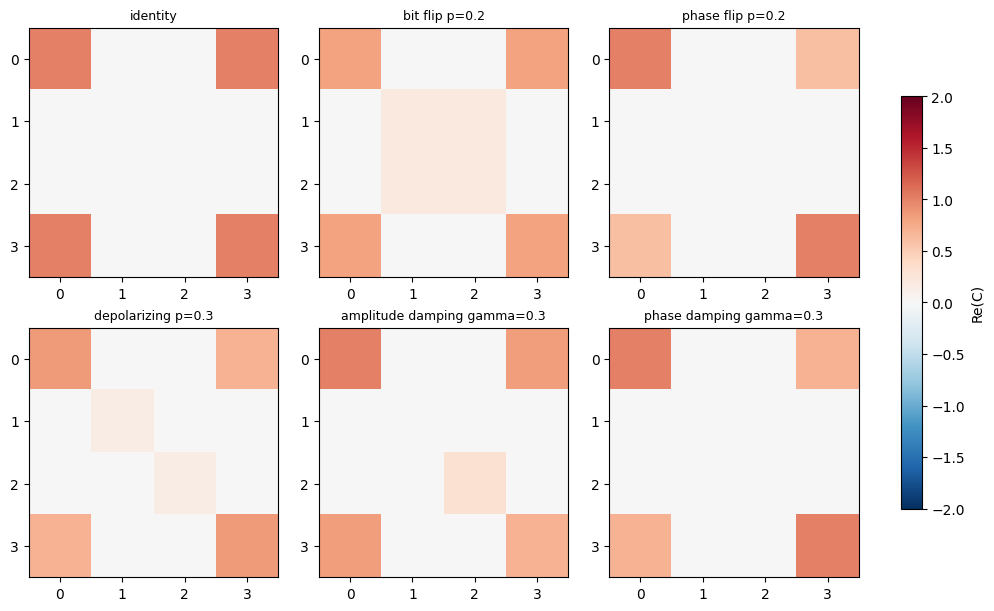
\includegraphics[width=0.94\textwidth]{fig_01_theory_01_cell6.png}
\caption{대표 qubit channel들의 Choi matrix 실수부. Identity는 rank-1 pure 구조, depolarizing은 대각이 균일해지고, amplitude damping은 비대칭 relaxation 구조로 나타난다. 앞 절의 닫힌 형이 이를 정량적으로 설명한다}
\label{fig:theory-choi-examples}
\end{figure}

그림 \ref{fig:theory-choi-examples}에서 identity의 Choi는 이상적 maximally entangled 구조(특정 위치에 큰 coherence)를, depolarizing은 maximally mixed로 밀리며 구조가 약해짐을 보인다(Bloch의 균일 수축과 동일한 내용이다). amplitude damping은 균일 수축으로 설명되지 않고, maximally mixed state조차 보존하지 않아 TP이지만 비-unital임을 확인할 수 있었다.

\begin{property}[TP $\neq$ unital]
$\E$ TP $\iff\Tr_B(C_\E)=I_A$; $\E$ unital $\iff\E(I)=I\iff\Tr_A(C_\E)=I_B$. Bloch에서 중심 이동 $\vec t\neq0$이 곧 비-unital성이라고 할 수 있다.
\end{property}

\subsection{수치 검증: ``오차 $10^{-16}$''의 의미}

\begin{mathbox}{machine precision}
배정밀도 단위 반올림은 $\varepsilon_{\mathrm{mach}}=2^{-52}\approx2.22\times10^{-16}$이다. 두 결과의 차이가 $\mathcal O(\varepsilon_{\mathrm{mach}})$이면 ``수치적으로 동일'', $\sim10^{-1}$이면 진짜 차이로 보았다(예: 뒤의 $-0.27$).
\end{mathbox}

\begin{table}[H]
\centering\small
\caption{이론 파트의 주요 수치 검증 결과}
\label{tab:theory-results}
\begin{tabularx}{\textwidth}{p{0.25\textwidth}p{0.31\textwidth}X}
\toprule
항목 & 관측값 & 해석(근거 식/정리) \\
\midrule
Identity channel & Choi rank $=1$ & $\rank(C_\E)=$ Kraus rank (정리 \ref{thm:cj}); noise 없음. \\
Depolarizing $p=0.3$ & min eig $=0.15$, TP=True, unital=True & $\min\mathrm{eig}=p/2=0.15\ge0$(CP); $\vec t=0$(unital). \\
Amplitude damping $\gamma=0.3$ & TP=True, unital=False, rank$=2$ & $\sum K_k^\dagger K_k=I$; $\vec t=(0,0,\gamma)\neq0$. \\
Random round-trip & error $\approx2.56\times10^{-16}$ & Choi$\to$Kraus$\to$action이 $\mathcal O(\varepsilon_{\mathrm{mach}})$로 일치. \\
Composition check & error $\approx2.48\times10^{-16}$ & $N_{\E_2\circ\E_1}=N_{\E_2}N_{\E_1}$(성질 \ref{prop:compose}). \\
\bottomrule
\end{tabularx}
\end{table}

표 \ref{tab:theory-results}을 한 줄씩 보면 다음과 같다. identity channel의 Choi rank가 1이라는 것은 noise 갈래가 없음을 뜻하므로 깨끗한 unitary임을 확인할 수 있었다. depolarizing의 최소 eigenvalue가 $0.15>0$이므로 모든 eigenvalue가 음이 아니어서 CP이고 unital도 True임을 확인할 수 있었다. amplitude damping은 TP=True이지만 unital=False로 나와, 앞 절에서 본 중심 이동을 수치가 그대로 확인할 수 있었다. 마지막 두 줄의 round-trip과 composition 오차가 $10^{-16}$ 수준이라는 것은 네 가지 표현이 서로 일치함을 의미한다고 생각된다.

\begin{remark}
perturbed identity는 Hermitian이고 $\Tr_B\approx I$여도 작은 음의 eigenvalue 하나로 CP=False가 된다. 정리 \ref{thm:cj}의 $C_\E\succeq0$은 거의 만족하는 정도로는 안 되고 정확히 만족해야 한다. 이는 뒤의 tomography에서 raw reconstruction을 그대로 믿으면 안 되는 이유라고 생각된다. shot noise가 비물리적(음의 eigenvalue) Choi를 만들면 CPTP projection이 필요하다.
\end{remark}

%==================================================================
\section{작업 2 --- Process Tomography와 Choi 재구성}
%==================================================================

\subsection{먼저 알아야 할 것: tomography가 필요한 이유}

이론적 Choi는 코드로 바로 계산할 수 있지만, 실제 장치에서 어떤 channel이 작용했는지는 직접 알 수 없다. $X$ gate를 실행해도 이상적 $X$ 뒤에 amplitude damping, depolarizing noise, coherent error가 섞일 수 있다.

\begin{conceptbox}{개념: process tomography}
의료 CT처럼 여러 각도의 정보를 합쳐 내부를 복원한다. 알 수 없는 channel에 정보적으로 완전한 입력 $\{\rho_a\}$를 넣고 출력 $\E(\rho_a)$를 측정한 뒤, linear 관계 $\E(\rho_a)=\Tr_A[(\rho_a^T\otimes I)C_\E]$(정리 \ref{thm:recover})를 $C_\E$에 대해 푼다(\textbf{linear inversion}).
\end{conceptbox}

\begin{definition}[CPTP projection]
shot noise로 $\widehat C\not\succeq0$일 때 가장 가까운 물리적 channel로 사영한다:
\[
C^\star=\arg\min_C\onenorm{C-\widehat C}\ \ \text{s.t.}\ \ C\succeq0,\ \Tr_B(C)=I_A,
\]
이는 볼록 최적화(SDP)이다. MLE는 같은 제약 아래 우도를 최대화하는 변형이라고 할 수 있다.
\end{definition}

재현성을 위해 실제 hardware 대신 offline simulated data를 사용했다(pipeline 검증 목적). 기준 gate는 그림 \ref{fig:qpt-target-circuits}이며, noise는 회로가 아니라 그 뒤의 Choi-level channel로 적용했다.

\begin{conceptbox}{개념: $X$, $H$, CNOT}
\textbf{$X$}: 양자 NOT($|0\rangle\leftrightarrow|1\rangle$). \textbf{$H$}: 균등 superposition을 만드는 Hadamard. \textbf{CNOT}: control $q_0$가 $|1\rangle$일 때만 target $q_1$을 뒤집는 2큐비트 entanglement gate. 앞 둘은 1큐비트, CNOT은 2큐비트라는 점이 뒤 결과 해석의 핵심이 된다.
\end{conceptbox}

\begin{figure}[H]
\centering
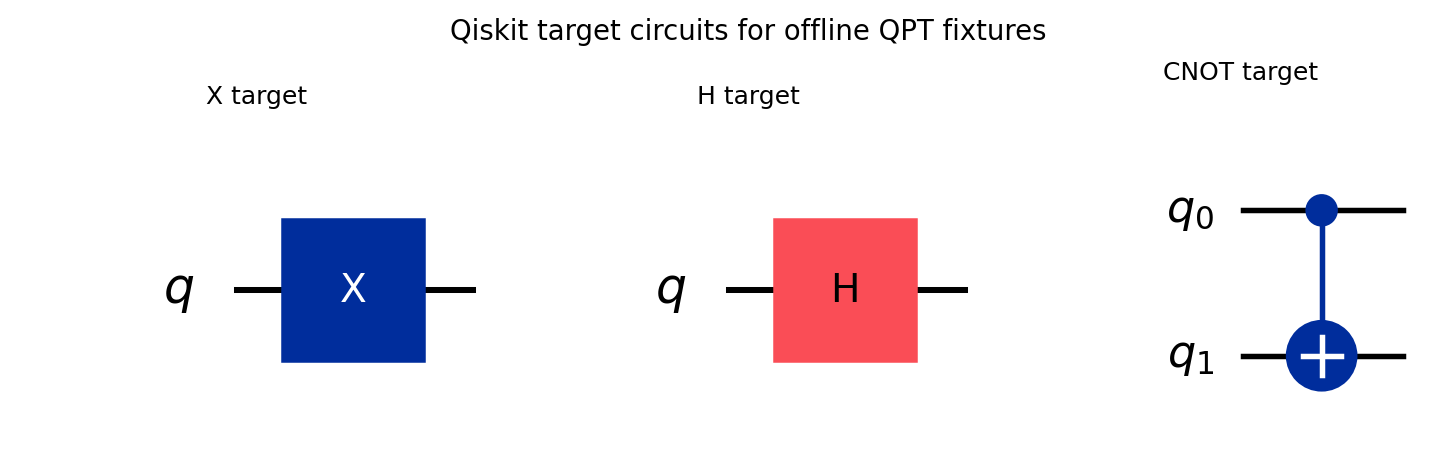
\includegraphics[width=0.92\textwidth]{fig_02_ibm_experiment_00_qiskit_circuits.png}
\caption{Offline QPT fixture의 target circuits. $X,H$는 1큐비트, CNOT은 2큐비트이다. Noise는 target gate 뒤의 Choi-level channel로 적용했다}
\label{fig:qpt-target-circuits}
\end{figure}

\subsection{비교 지표: fidelity와 diamond distance}

\begin{definition}[process fidelity]
$F(\rho,\sigma)=(\Tr\sqrt{\sqrt\rho\sigma\sqrt\rho})^2$. channel의 process fidelity는 정규화 Choi state $\rho_\E=C_\E/d_A$로 $F_{\mathrm{pro}}(\E,\mathcal F)=F(\rho_\E,\rho_{\mathcal F})$ (entanglement fidelity와 동치).
\end{definition}

\begin{theorem}[average gate fidelity 관계]\label{thm:favg}
$\boxed{F_{\mathrm{avg}}=\dfrac{dF_{\mathrm{pro}}+1}{d+1}}$ (Horodecki--Nielsen).
\end{theorem}

\begin{mathbox}{표 \ref{tab:qpt-results}의 수치 재현}
정리 \ref{thm:favg}로 표의 값을 그대로 계산할 수 있었다.
\begin{align*}
X\,(d{=}2):&\ \tfrac{2(0.959583)+1}{3}=0.973055,\quad
H\,(d{=}2):\ \tfrac{2(0.94)+1}{3}=0.960000,\\
\mathrm{CNOT}\,(d{=}4):&\ \tfrac{4(0.92)+1}{5}=0.936000.
\end{align*}
즉 표의 두 fidelity는 한 공식으로 서로 묶여 있다고 할 수 있다.
\end{mathbox}

\begin{definition}[diamond norm]
$\diamondnorm{\Delta}=\max_{\rho\in\Dens(\Hcal_A\otimes\Hcal_R)}\onenorm{(\Delta\otimes\id_R)(\rho)}$, $\dim\Hcal_R=\dim\Hcal_A$ (최댓값은 pure state에서 달성). half-diamond distance $=\tfrac12\diamondnorm{\E_0-\E_1}$.
\end{definition}

\begin{intuitionbox}
\textbf{fidelity 대 diamond:} fidelity는 Choi state끼리의 평균적 겹침이고, diamond는 최악의 입력(entanglement 허용)에서의 차이이다. $X$가 $F_{\mathrm{pro}}=0.96$로 평균적으로 비슷해도 half-diamond $=0.08\neq0$로, 최악에서는 구별됨을 알 수 있었다.
\end{intuitionbox}

\subsection{이상적 Choi 대 재구성된 Choi}

\begin{figure}[H]
\centering
\begin{subfigure}{0.48\textwidth}\centering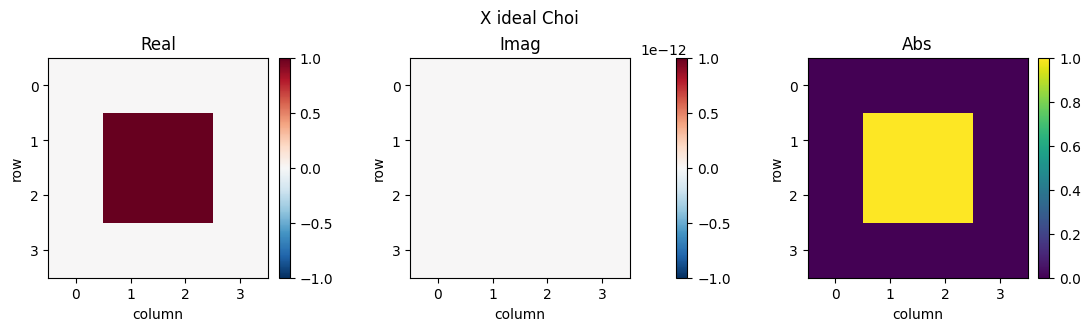
\includegraphics[width=\textwidth]{fig_02_ibm_experiment_01_cell20.png}\caption{$X$ ideal Choi}\end{subfigure}\hfill
\begin{subfigure}{0.48\textwidth}\centering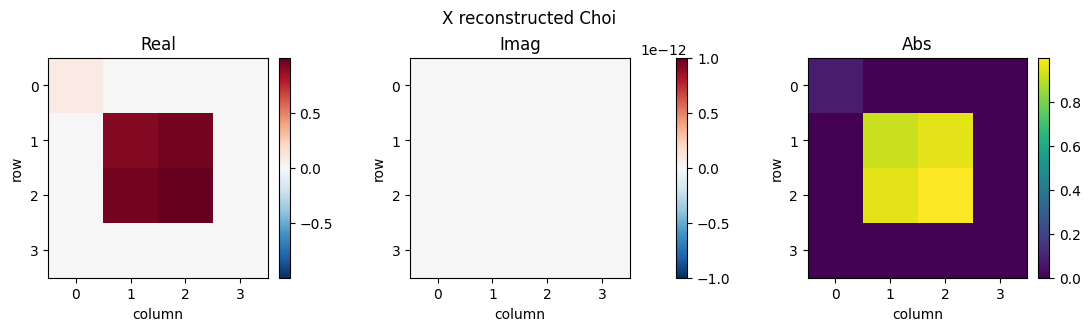
\includegraphics[width=\textwidth]{fig_02_ibm_experiment_02_cell20.png}\caption{$X$ reconstructed Choi}\end{subfigure}
\caption{$X$의 ideal/reconstructed Choi. 큰 구조는 유지되되 ideal pattern을 벗어난 작은 성분이 나타난다. 이는 이상적 unitary에 noise가 더해진 형태라고 생각된다}
\label{fig:qpt-x-choi}
\end{figure}

두 행렬이 완전히 같다면 $F_{\mathrm{pro}}=1$, half-diamond $=0$이어야 한다. 측정한 결과는 $F_{\mathrm{pro}}=0.959583$, half-diamond $=0.080000$으로 나타났다. 이를 통해 평균적으로는 비슷하지만 최악에서는 차이가 남는 구도를 확인할 수 있었다.

\begin{figure}[H]
\centering
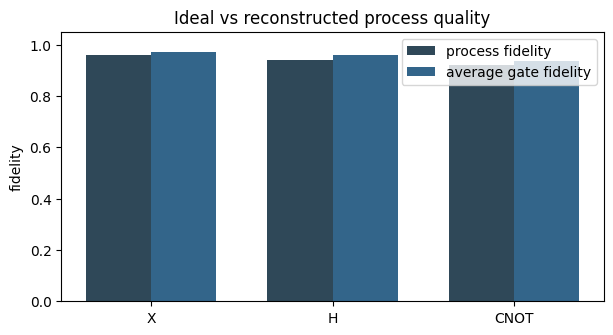
\includegraphics[width=0.74\textwidth]{fig_02_ibm_experiment_10_cell24.png}
\caption{$X,H,$CNOT의 process/average gate fidelity. 모두 $1$보다 작아 noise가 존재하며, CNOT이 가장 낮게 나타났다}
\label{fig:qpt-fidelity-bars}
\end{figure}

\begin{remark}[차원이 커지면 왜 나빠지나]
CNOT은 2큐비트라 $C_\E\in\Lin(\mathbb C^{16})$이고, 전역 depolarizing의 Pauli error 갈래 수는 $d^2-1=15$로 1큐비트의 $3$보다 많다. 이에 같은 세기라도 오차가 더 많은 방향으로 분산되어 $F_{\mathrm{pro}}$가 낮아진다고 생각된다.
\end{remark}

\subsection{noise의 방향성: Bloch affine 진단}

\begin{definition}[잔차 channel의 affine 진단]
잔차를 $\vec r\mapsto M\vec r+\vec t$로 보고 $M=U\Sigma V^\dagger$, $\Sigma=\mathrm{diag}(s_1,s_2,s_3)$로 둔다. 다음과 같이 분류한다.
\[
\|\vec t\|_2>\tau\Rightarrow\text{relaxation-like},\quad
\|\vec t\|_2\approx0\ \&\ \mathrm{spread}(s_i)\approx0\Rightarrow\text{depolarizing-like},
\]
이때 $\mathrm{spread}=\max_i s_i-\min_i s_i$, $\tau=0.05$로 두었다.
\end{definition}

\begin{figure}[H]
\centering
\begin{subfigure}{0.47\textwidth}\centering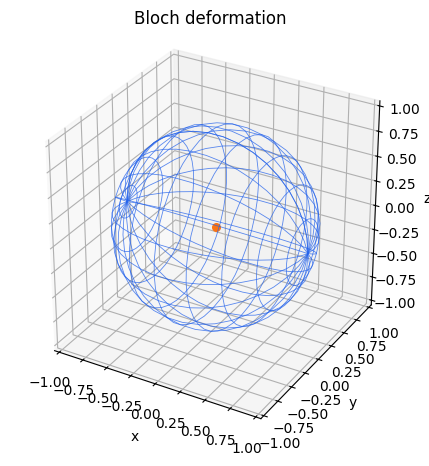
\includegraphics[width=0.82\textwidth]{fig_02_ibm_experiment_07_cell22.png}\caption{$X$ reconstructed}\end{subfigure}\hfill
\begin{subfigure}{0.47\textwidth}\centering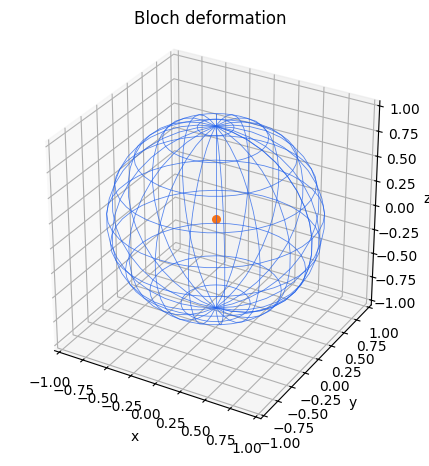
\includegraphics[width=0.82\textwidth]{fig_02_ibm_experiment_08_cell22.png}\caption{$H$ reconstructed}\end{subfigure}
\caption{재구성된 1큐비트 channel의 Bloch 변형. depolarizing-like는 균일 수축($\vec t\approx0$), amplitude-damping-like는 중심 이동($\vec t\neq0$). fidelity 숫자만으로 안 보이는 방향성을 보여준다}
\label{fig:qpt-bloch}
\end{figure}

그림 \ref{fig:qpt-bloch}은 fidelity만으로는 설명하기 어려운 부분을 보완한다. fidelity는 하나의 숫자로 평균적 유사도를 말해 주지만, noise가 어느 방향으로 작용하는지는 직접 보여주지 않는다. 반면 Bloch 변형을 보면 구가 균일하게 줄어드는지, 특정 방향으로 이동하는지를 확인할 수 있었다. 이 진단은 그림만 보고 정성적으로 붙인 것이 아니다. 재구성된 Choi를 Pauli-transfer 표현으로 바꾼 뒤 affine action을 계산하여 얻었다.

\begin{table}[H]
\centering\small
\caption{1큐비트 재구성 channel의 Bloch affine 진단. $H$의 $10^{-15},10^{-12}$는 사실상 $0$으로 보았다}
\label{tab:qpt-bloch-diagnostics}
\begin{tabularx}{\textwidth}{lcccX}
\toprule
Gate & $\|\vec t\|_2$ & SV spread & Mean shrinkage & 진단 근거 \\
\midrule
$X$ & 0.07999965 & 0.03916625 & 0.94611071 & $\|\vec t\|_2>0.05\Rightarrow$ relaxation-like. \\
$H$ & $1.999\times10^{-15}$ & $1.999\times10^{-12}$ & 0.92000000 & $\|\vec t\|_2,\mathrm{spread}\approx\mathcal O(\varepsilon)\Rightarrow$ isotropic depolarizing-like. \\
\bottomrule
\end{tabularx}
\end{table}

표 \ref{tab:qpt-bloch-diagnostics}을 보면 $X$는 중심 이동 $\|\vec t\|_2\approx0.08$로 기준값 $0.05$보다 크므로 relaxation으로 분류되었다. $H$는 $\|\vec t\|_2$가 $10^{-15}$로 사실상 0이고 축별 차이도 $10^{-12}$로 0이며 전체 수축만 뚜렷하므로 depolarizing으로 분류할 수 있었다. 이에 따라 tomography는 세 가지를 함께 보아야 안정적으로 해석된다고 생각된다: heatmap은 구조적 차이를, fidelity는 한 숫자 요약을, Bloch는 물리적 noise 모양을 보여준다. 세 관찰을 종합한 값이 표 \ref{tab:qpt-results}이다.

\begin{table}[H]
\centering\small
\caption{Offline simulated QPT 결과 ($F_{\mathrm{avg}}$는 정리 \ref{thm:favg}로 유도)}
\label{tab:qpt-results}
\begin{tabularx}{\textwidth}{lcccX}
\toprule
Gate & $F_{\mathrm{pro}}$ & $F_{\mathrm{avg}}$ & Half-diamond & 진단 \\
\midrule
$X$ & 0.959583 & 0.973055 & 0.080000 & amplitude-damping-like relaxation \\
$H$ & 0.940000 & 0.960000 & 0.060000 & depolarizing-like isotropic shrinkage \\
CNOT & 0.920000 & 0.936000 & 0.080000 & stochastic global depolarizing-like noise \\
\bottomrule
\end{tabularx}
\end{table}

\begin{remark}[비물리적 재구성]
linear inversion perturbation의 최소 eigenvalue $-0.270000$은 $\mathcal O(\varepsilon_{\mathrm{mach}})$가 아닌 진짜 음수이다(정리 \ref{thm:cj} 위반). 이에 raw reconstruction은 물리적 channel로 받아들이기 어렵고, CPTP projection으로 $C^\star\succeq0$을 회복해야 한다. 이는 결과를 보기 좋게 만드는 후처리가 아니다. density matrix와 channel이 반드시 만족해야 하는 물리 법칙(eigenvalue $\ge0$)을 회복하는 과정이라고 생각된다.
\end{remark}

%==================================================================
\section{작업 3 --- Channel Discrimination, diamond norm, SDP}
%==================================================================

\subsection{먼저 알아야 할 것: 구별과 비슷함은 다른 문제}

fidelity는 평균적 유사도를 말해 준다. 그러나 두 channel을 실제로 얼마나 잘 구별하는가는 별개의 문제이다. 동전을 던져 $\E_0,\E_1$ 중 하나를 주면, 원하는 입력으로 측정해 어느 쪽인지 맞히는 게임을 생각할 수 있다.

\begin{theorem}[Holevo--Helstrom]\label{thm:helstrom}
사전확률 $\tfrac12$씩으로 두 상태 $\rho_0,\rho_1$를 구별하는 최적 성공확률은
\[
p_{\mathrm{succ}}^{\max}=\tfrac12+\tfrac14\onenorm{\rho_0-\rho_1}=\tfrac12+\tfrac12T(\rho_0,\rho_1),
\]
최적 측정은 $\rho_0-\rho_1$의 양/음 고유공간 사영이다. 이때 $T(\rho_0,\rho_1)=\tfrac12\onenorm{\rho_0-\rho_1}$.
\end{theorem}
\begin{proof}[증명 개요]
POVM $\{M,I-M\}$의 성공확률은 $\tfrac12+\tfrac12\Tr[M\Delta]$, $\Delta=\Delta_+-\Delta_-$이다. $\Tr[M\Delta]\le\Tr\Delta_+=\tfrac12\onenorm\Delta$이고, $M=\Delta_+$ 사영에서 등호가 성립한다.
\end{proof}

\begin{theorem}[channel 구별과 diamond norm]\label{thm:chandisc}
$\E_0,\E_1$을 한 번 사용해 구별하는 최적 성공확률(reference system 허용)은
\[
\boxed{p_{\mathrm{succ}}^{\max}=\tfrac12+\tfrac14\diamondnorm{\E_0-\E_1}.}
\]
\end{theorem}
\begin{proof}[증명 개요]
입력 $|\psi\rangle\in\Hcal_A\otimes\Hcal_R$에 정리 \ref{thm:helstrom}을 적용하면 성공확률은 $\tfrac12+\tfrac14\onenorm{(\Delta\otimes\id_R)(|\psi\rangle\langle\psi|)}$이고, $|\psi\rangle$로 최대화하면 $=\diamondnorm\Delta$이다.
\end{proof}

\begin{mathbox}{왜 reference system(ancilla)이 도움이 되는가}
$\diamondnorm{}$의 최댓값이 entangled $|\psi\rangle$에서 달성될 수 있기 때문이다. 단독 입력만 쓰면 더 작은 값만 얻는다:
\[
\max_{\rho\in\Dens(\Hcal_A)}\onenorm{\Delta(\rho)}\ \le\ \diamondnorm{\Delta},
\]
이때 부등호가 엄격할 수 있다. 이는 표 \ref{tab:sdp-results}의 $0.750\to0.875$ 향상의 근원이라고 할 수 있다.
\end{mathbox}

\begin{theorem}[Watrous SDP]\label{thm:sdp}
$\Delta$의 Choi $J=C_\Delta$($A$ 입력)에 대해
\[
\diamondnorm{\Delta}=\max_{W,\rho}\langle J,W\rangle\quad\text{s.t.}\quad0\preceq W\preceq\rho\otimes I_B,\ \rho\in\Dens(\Hcal_A),
\]
변수 $W\succeq0,\rho\succeq0$의 볼록 문제로 효율적으로 풀린다 (Watrous 2009/2012).
\end{theorem}

\begin{conceptbox}{개념: SDP가 자연스러운 이유}
물리적으로 가능한 대상은 모두 $\succeq0$ 제약으로 표현되므로, 최적 전략 찾기가 $\succeq0$ 아래 선형 목적 최적화(SDP)가 된다. 이때 \textbf{Choi matrix $J$가 SDP의 입력 데이터}라는 점이 핵심이라고 할 수 있다. Choi가 operational한 양과 직결되는 통로가 된다.
\end{conceptbox}

\subsection{수치 결과}

먼저 가장 해석하기 쉬운 경우로 depolarizing channel의 parameter가 바뀔 때 성공확률이 어떻게 변하는지 보았다. 이 예시는 두 channel의 차이가 커질수록 구별이 쉬워진다는 기본 직관을 확인하는 역할을 한다.

\begin{figure}[H]
\centering
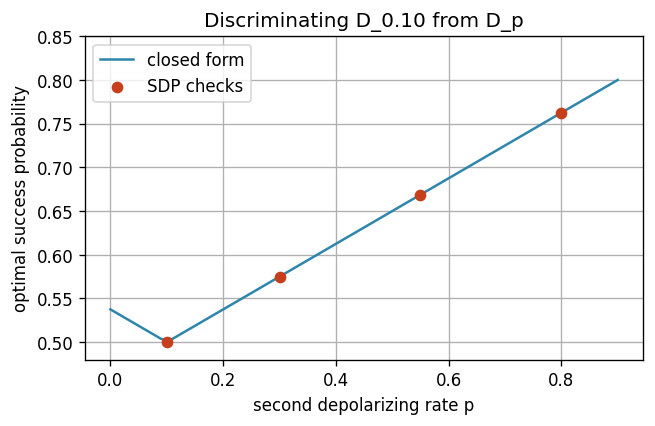
\includegraphics[width=0.72\textwidth]{fig_03_sdp_discrimination_01_cell9.png}
\caption{Depolarizing parameter 차이에 따른 구별 success probability. 차이가 $0$이면 $p\to\tfrac12$(찍기), 커지면 정리 \ref{thm:chandisc}에 따라 $p$가 증가한다}
\label{fig:sdp-depolarizing}
\end{figure}

그림 \ref{fig:sdp-depolarizing}에서 성공확률이 $0.5$ 근처라는 것은 찍기와 큰 차이가 없음을 뜻한다. 기준 channel과 비교 channel의 depolarizing 세기가 거의 같으면 출력 상태의 차이가 작아져 구별이 어려워진다고 생각된다. 반대로 parameter 차이가 커질수록 출력 상태들이 더 많이 달라지고, 이에 따라 최적 측정의 성공확률도 증가함을 확인할 수 있었다.

\begin{figure}[H]
\centering
\begin{subfigure}{0.48\textwidth}\centering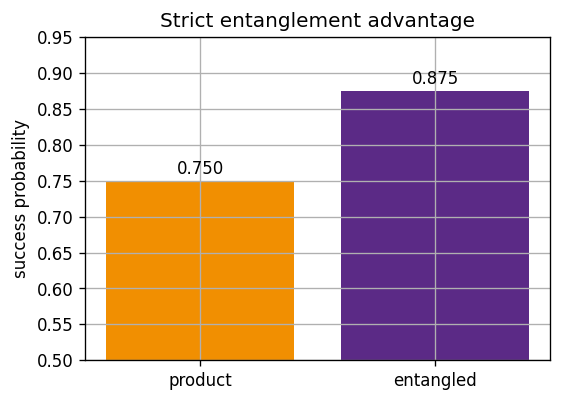
\includegraphics[width=\textwidth]{fig_03_sdp_discrimination_04_cell18.png}\caption{Product vs entangled}\end{subfigure}\hfill
\begin{subfigure}{0.48\textwidth}\centering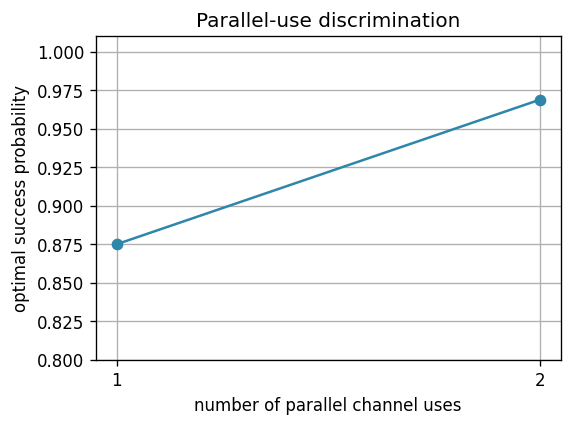
\includegraphics[width=\textwidth]{fig_03_sdp_discrimination_05_cell21.png}\caption{Parallel use}\end{subfigure}
\caption{entanglement과 반복 사용의 이점. product $0.750000$, ancilla-assisted $0.875000$, 2-shot parallel $0.968750$으로 나타났다}
\label{fig:sdp-advantage}
\end{figure}

단독 입력과 entangled 입력의 차이는 실제로 구별 성능을 끌어올리는 operational advantage로 나타났다. reference system과 entanglement을 만들면 channel 작용이 joint state의 correlation에도 흔적을 남겨, 그 추가 정보로 성공확률이 오른다($0.75\to0.875$). 더불어 2-shot 결과가 $0.968750$까지 오른 것도 자연스럽다고 생각된다. 같은 channel을 여러 번 쓸 수 있으면 한 번의 출력보다 더 많은 정보를 얻고, 두 channel의 차이가 누적되기 때문이다.

\begin{property}[병렬 사용은 곱 channel의 diamond norm]
$n$번 병렬 사용 전략의 성공확률은 $\tfrac12+\tfrac14\diamondnorm{\E_0^{\otimes n}-\E_1^{\otimes n}}$로 차이가 누적된다. 다만 차원이 $d_A^n$으로 지수적으로 증가하여 SDP 비용이 급증한다.
\end{property}

\begin{table}[H]
\centering
\caption{SDP 기반 channel discrimination 결과}
\label{tab:sdp-results}
\begin{tabular}{lcc}
\toprule
전략 & 성공확률 & 근거 \\
\midrule
Bit-flip closed-form 검증 & 0.625000 & 해석적 $\diamondnorm{}$와 SDP(정리 \ref{thm:sdp}) 일치 → 구현 신뢰성. \\
Product input & 0.750000 & $\max_\rho\onenorm{\Delta(\rho)}$ (reference 없음). \\
Ancilla-assisted input & 0.875000 & 전체 $\diamondnorm{\Delta}$ (정리 \ref{thm:chandisc}). \\
2-shot parallel & 0.968750 & 차이 누적. \\
\bottomrule
\end{tabular}
\end{table}

표 \ref{tab:sdp-results}의 첫 줄($0.625$)은 손으로 풀 수 있는 bit-flip(예제 \ref{ex:bitflip}의 channel)의 해석적 diamond norm과 SDP 수치가 일치함을 확인한 것으로, 구현 자체가 옳음을 알 수 있었다. 이후 $0.750\to0.875\to0.969$의 단조 증가는 reference 없음 $\to$ entanglement $\to$ 반복에 대응한다고 할 수 있다.

%==================================================================
\section{작업 4 --- Non-Markovian Dynamics와 Quantum Combs}
%==================================================================

\subsection{먼저 알아야 할 것: 단일 시점 channel의 한계}

지금까지의 Choi는 하나의 입력-출력 관계를 설명했다. 그러나 시간 과정에서 계가 environment와 여러 번 상호작용하고 그 environment가 다음 시점에도 기억을 남기면 단일 channel로 설명되지 않는다.

\begin{conceptbox}{개념: Markovian 대 non-Markovian}
\textbf{Markovian}은 기억 없는 과정으로, environment로 새어 나간 정보가 돌아오지 않는다. \textbf{non-Markovian}은 environment에 저장된 정보가 계로 되돌아올 수 있다. 각 시점 marginal이 멀쩡한 CPTP라도 시점 간 correlation이 남으면 전체는 기억 없는 곱으로 분해되지 않는다.
\end{conceptbox}

\begin{definition}[dynamical map과 CP-divisibility]
시간 channel 족 $\{\Lambda(t)\}$($\Lambda(0)=\id$)에서 중간 전파자 $V(t,s)$를 $\Lambda(t)=V(t,s)\Lambda(s)$로 정의한다. 모든 $t\ge s$에서 $V(t,s)$가 CP이면 \textbf{CP-divisible}(Markovian)이라 한다.
\end{definition}

\begin{property}[CPTP의 trace-distance 수축성]\label{prop:contract}
CPTP $\Lambda$와 두 상태에 대해 $T(\Lambda\rho,\Lambda\sigma)\le T(\rho,\sigma)$이다. 즉 물리적(CP) 진화는 구별 가능성을 증가시키지 못한다.
\end{property}

\begin{intuitionbox}
\textbf{직관(성질 \ref{prop:contract}의 위력):} trace distance가 다시 증가하면, 그 구간의 중간 전파자는 CP일 수 없다. 이는 정보가 environment에서 계로 되돌아온 것으로, 기억 효과의 신호라고 생각된다.
\end{intuitionbox}

\begin{conceptbox}{개념: trace distance와 BLP measure}
\textbf{trace distance} $T=\tfrac12\onenorm{\rho-\sigma}$는 두 상태의 구별 가능성을 나타낸다(0이면 구별 불가). noise는 보통 $T$를 단조 감소시키지만, 다시 증가하면 기억 효과의 증거가 된다.
\end{conceptbox}

\begin{definition}[BLP measure]
$\sigma(t)=\frac{d}{dt}T(\Lambda(t)\rho_1,\Lambda(t)\rho_2)$일 때 $\mathcal N_{\mathrm{BLP}}=\max_{\rho_1,\rho_2}\int_{\sigma(t)>0}\sigma(t)\,dt$. $>0$이면 non-Markovian이다.
\end{definition}

\begin{conceptbox}{개념: RHP-style witness}
RHP는 중간 전파자 $V(t+\epsilon,t)$의 CP성을 직접 본다. $g(t)=\lim_{\epsilon\to0^+}\frac1\epsilon(\onenorm{(\id\otimes V(t+\epsilon,t))|\Omega\rangle\langle\Omega|}-1)$이 $V$가 CP인 동안 $0$, 깨지면 $>0$이 된다. 이를 적분한 것이 RHP-style witness이다. BLP가 정보 역류를, RHP가 중간 단계의 비-CP성을 본다고 할 수 있다.
\end{conceptbox}

\begin{figure}[H]
\centering
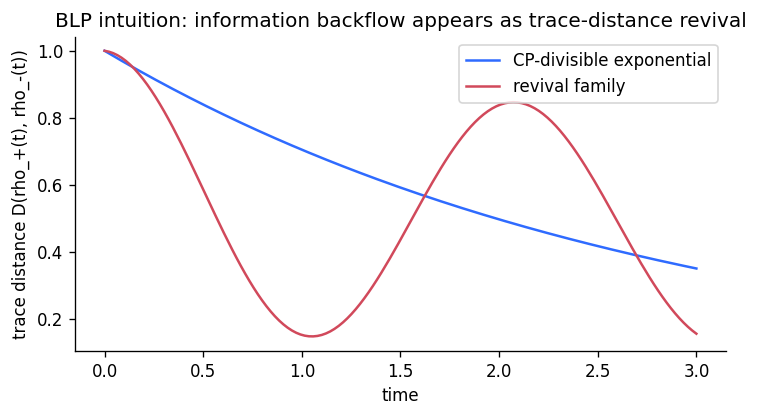
\includegraphics[width=0.76\textwidth]{fig_04_quantum_combs_01_cell7.png}
\caption{trace distance의 시간 변화. Markovian dephasing은 단조 감소($\sigma\le0$, 성질 \ref{prop:contract}와 부합)하지만, revival dephasing은 다시 증가($\sigma>0$)하여 $\mathcal N_{\mathrm{BLP}}>0$. 정보가 environment에서 system으로 되돌아온 것으로 생각된다}
\label{fig:comb-trace-distance}
\end{figure}

그림 \ref{fig:comb-trace-distance}에서 exponential dephasing의 trace distance는 계속 줄어든다. 이는 두 상태를 구별할 정보가 시간이 지나며 줄어드는 상황이라고 할 수 있다. 반대로 revival dephasing에서는 trace distance가 다시 증가하는 구간이 나타나는데, 이는 이전에 environment로 흘러나갔던 정보가 일부 되돌아온 것이라고 생각된다.

\subsection{구조적 증거: comb와 memoryless product}

trace distance 곡선만으로는 다중 시점 과정 전체의 구조를 직접 볼 수 없다. 이에 전체 two-use 과정을 하나의 comb로 놓고 기억 없는 곱과 비교했다.

\begin{conceptbox}{개념: quantum comb}
여러 time slot의 입력-출력을 하나의 큰 Choi-like operator로 묶은 것이다. 이름이 빗(comb)인 것은 시간 축을 따라 단자(이빨)가 늘어선 모양 때문이라고 할 수 있다. 단일 channel에서는 안 보이는 시간 correlation과 기억 잔여물을 드러낸다.
\end{conceptbox}

\begin{definition}[quantum comb의 인과 위계]
$N$-comb은 $\bigotimes_k\Hcal_k$(번갈아 in/out) 위 $C\succeq0$이다. 2-comb은
\[
\Tr_3 C=I_2\otimes C^{(1)},\qquad \Tr_1 C^{(1)}=I_0
\]
를 만족한다(Chiribella--D'Ariano--Perinotti). 이는 정리 \ref{thm:cj}의 TP($\Tr_B C_\E=I_A$)를 여러 시점으로 확장한 것이라고 할 수 있다.
\end{definition}

\begin{definition}[link product과 correlation norm]
comb 합성은 공유 계의 partial trace와 transpose를 결합한 \textbf{link product} $\star$로 주어진다. 기억 없는 과정은 $C_{\mathrm{prod}}=\bigotimes_k C^{(k)}$로 분해되고, relative correlation norm
\[
\eta=\frac{\onenorm{C-C_{\mathrm{prod}}}}{\onenorm{C}}
\]
이 $\neq0$이면 시점 간 correlation(기억)이 존재한다.
\end{definition}

\begin{conceptbox}{개념: collision model}
계가 environment 입자들과 차례로 충돌하는데, 같은 environment를 재사용하면 첫 충돌의 흔적이 다음 충돌에 영향을 준다. 즉 environment 재사용이 기억의 원천이 된다.
\end{conceptbox}

\begin{figure}[H]
\centering
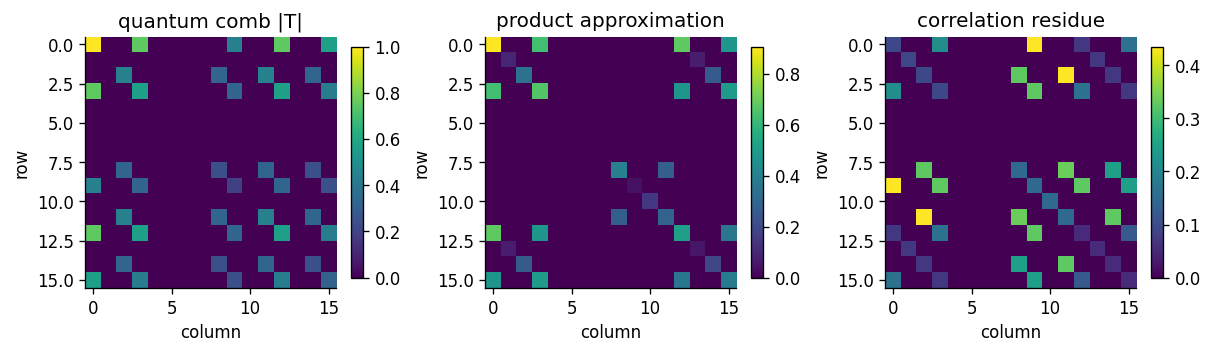
\includegraphics[width=0.92\textwidth]{fig_04_quantum_combs_02_cell10.png}
\caption{Two-use collision model의 comb(좌), memoryless product(중), 그리고 둘의 차이(우). 차이가 $0$이 아니면 시점 간 correlation이 존재함을 뜻하며, 독립적 두 channel의 연속으로 설명되지 않는다고 생각된다}
\label{fig:comb-correlation}
\end{figure}

\begin{mathbox}{collision model의 수치 검증}
$C\in\Lin(\mathbb C^{16})$, 최소 eigenvalue $-1.774\times10^{-16}=\mathcal O(\varepsilon_{\mathrm{mach}})\Rightarrow C\succeq0$(물리적). 인과 위계=True. 그러나 곱 분해 가능성=False, $\eta=\onenorm{C-C_{\mathrm{prod}}}/\onenorm{C}\approx0.5307\neq0$. \textbf{이 $\eta\neq0$이 기억 효과의 정량적 핵심 증거이다.}
\end{mathbox}

기억은 각 시점 marginal 자체보다 시점 간 correlation에서 나온다고 생각된다. 다음 그림이 이를 보여준다.

\begin{figure}[H]
\centering
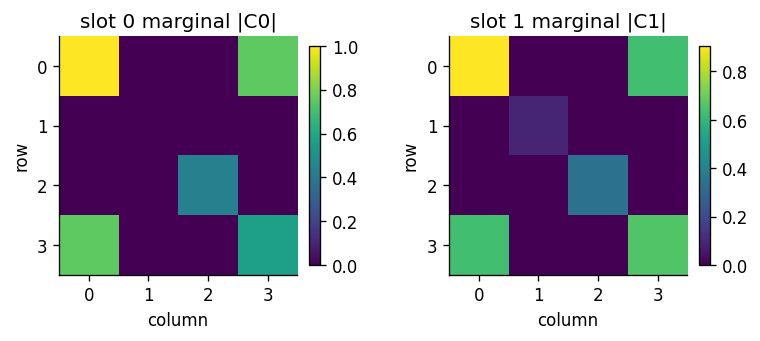
\includegraphics[width=0.72\textwidth]{fig_04_quantum_combs_03_cell13.png}
\caption{각 slot의 marginal Choi. 개별로는 정상적인 1단계 channel처럼 보이나, 곱만으로는 전체 comb를 복원할 수 없었다($\eta\neq0$). 매 시점 멀쩡한 channel을 얻어도 전체가 Markovian이라 결론낼 수 없음을 알 수 있었다}
\label{fig:comb-marginals}
\end{figure}

\begin{table}[H]
\centering
\caption{비마르코프성 witness 결과. 정의가 다른 두 진단이 같은 결론으로 나타났다}
\label{tab:nonmarkov-results}
\begin{tabular}{lcc}
\toprule
Channel family & BLP grid estimate & RHP-style grid witness \\
\midrule
Exponential dephasing & 0.000000 & 0.000000 \\
Revival dephasing & 0.699240 & 0.896321 \\
\bottomrule
\end{tabular}
\end{table}

표 \ref{tab:nonmarkov-results}에서 exponential dephasing은 $\mathcal N_{\mathrm{BLP}}=0$, RHP$=0$으로 CP-divisible임을 확인할 수 있었다. 반면 revival dephasing은 둘 다 양수로, 정의가 서로 다른 두 measure가 동일하게 non-Markovian을 가리켰다. 이를 통해 결과가 robust함을 확인할 수 있었다.

%==================================================================
\section{작업 5 --- Interactive Widget과 조건의 시각적 동치}
%==================================================================

Widget은 정리 \ref{thm:cj}의 두 조건을 실시간으로 보여준다. 수식으로 $C_\E\succeq0$, $\Tr_B(C_\E)=I_A$는 간단해 보이지만, channel 작용에서 어떤 모양인지 곧바로 떠올리기는 쉽지 않다. 이에 parameter를 움직이면 다음이 동시에 갱신되도록 구성했다.
\[
\underbrace{\text{Choi eigenspectrum}}_{C_\E\succeq0?\ (\text{CP})},\quad
\underbrace{\Tr_B(C_\E)}_{=I_A?\ (\text{TP})},\quad
\underbrace{\text{Kraus }\{K_k\}}_{\text{정리 \ref{thm:cj}}},\quad
\underbrace{\vec r\mapsto M\vec r+\vec t}_{\text{Bloch}}.
\]

앞 네 작업은 Choi를 따로 사용했지만, widget은 이들을 한 화면에서 연결한다. amplitude damping을 고르면 Choi 패턴과 eigenvalue뿐 아니라 Bloch가 어느 방향으로 변형되는지도 동시에 볼 수 있었다.

\begin{figure}[H]
\centering
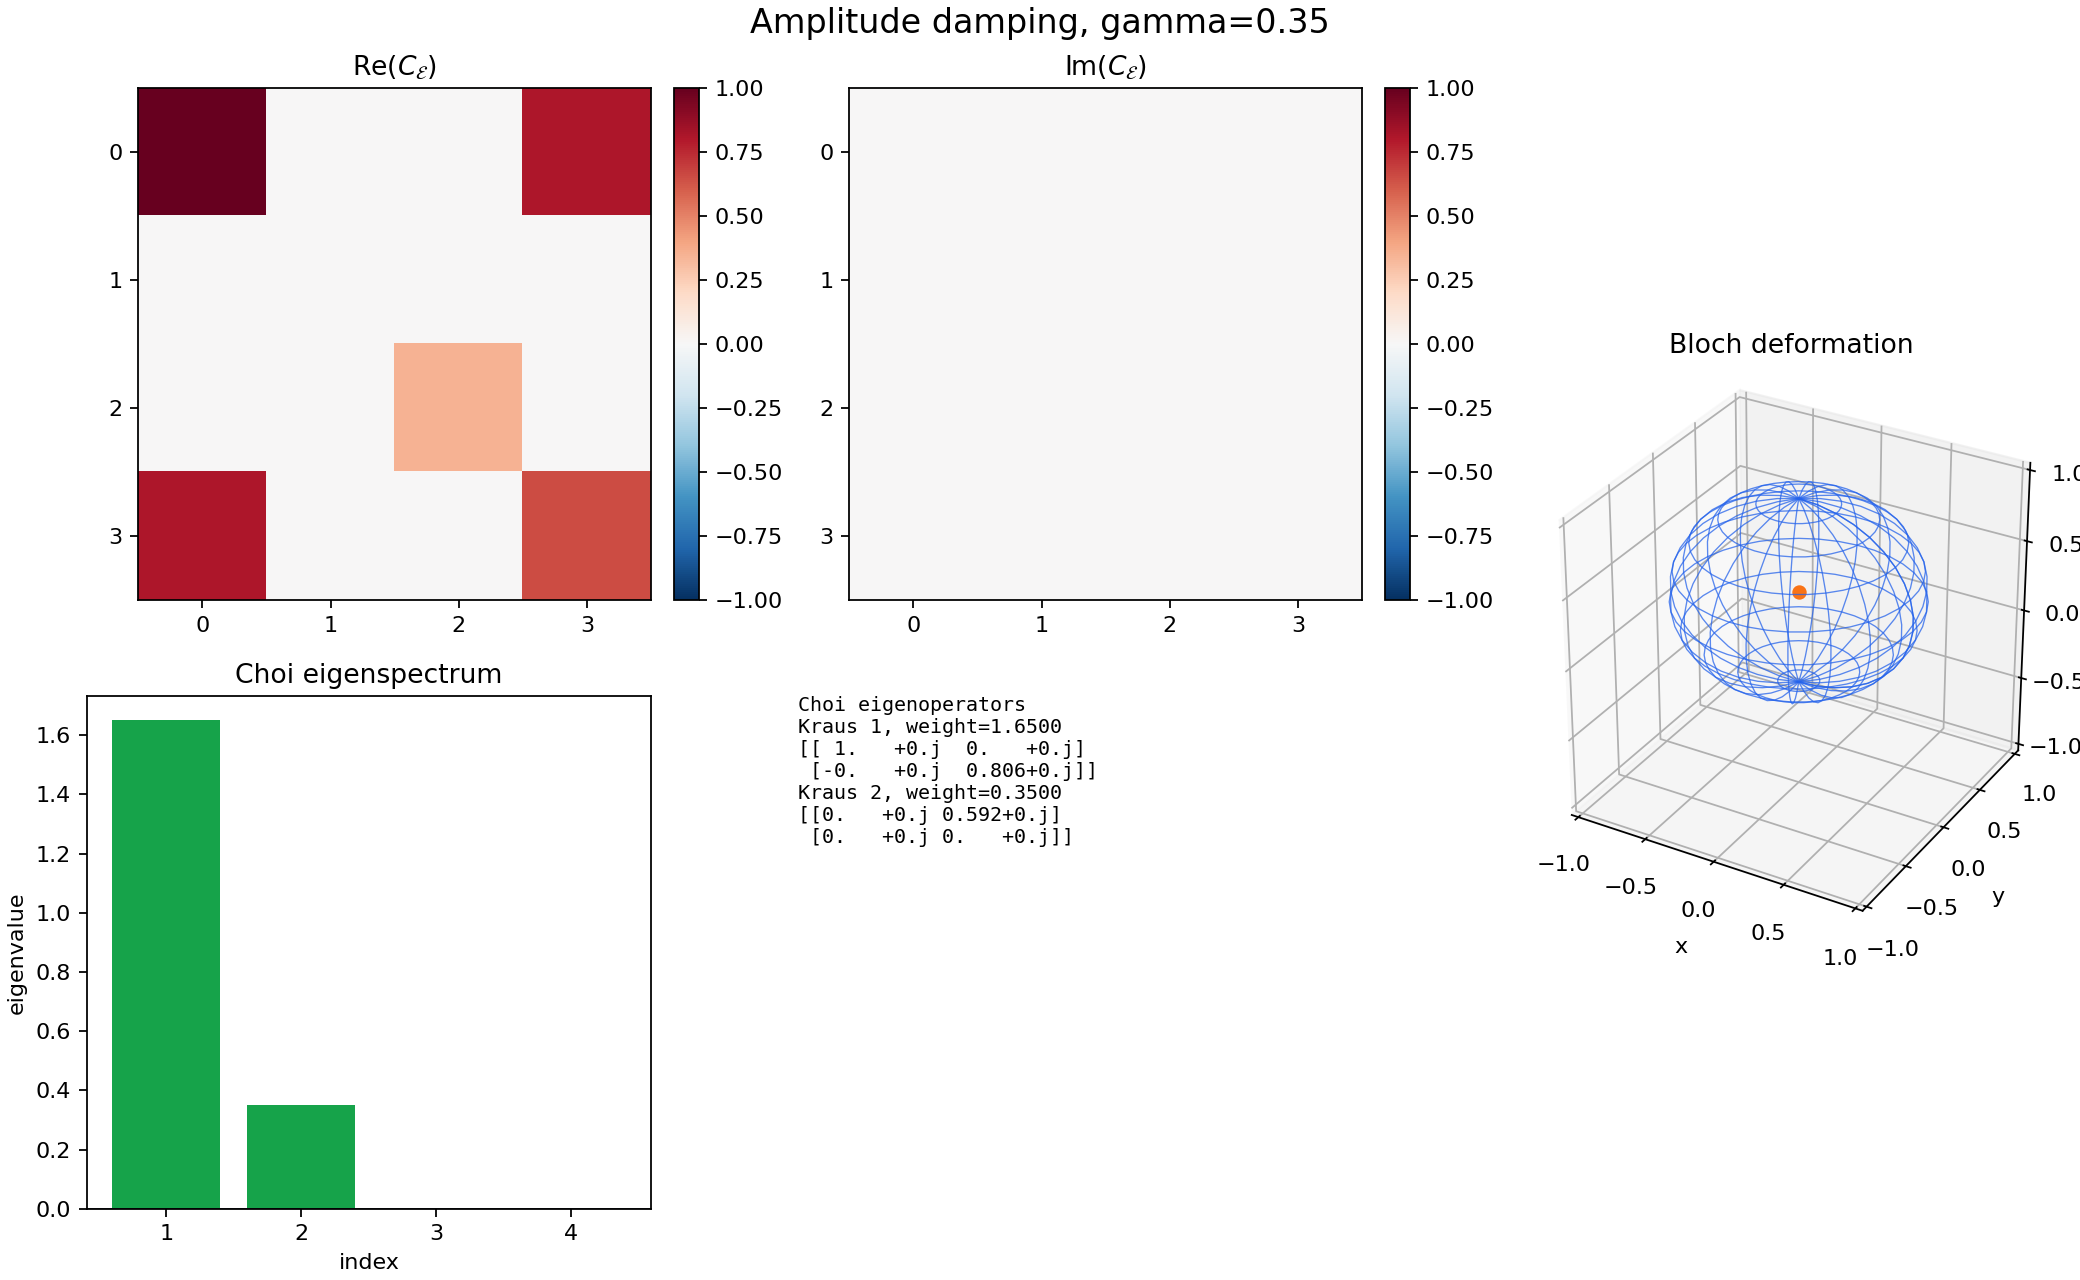
\includegraphics[width=0.94\textwidth]{fig_widget_dashboard.png}
\caption{amplitude damping 예시. Choi 실수부/허수부/절댓값(좌), Choi eigenvalue와 Bloch 변형(우). $\vec t=(0,0,\gamma)\neq0$이라 중심이 이동하며, 이는 비-unital성의 시각적 표현이라고 할 수 있다}
\label{fig:widget-dashboard}
\end{figure}

\begin{property}[CP 경계의 시각적 신호]
parameter를 CP 영역 밖으로 옮기면 $C_\E$에 음의 eigenvalue가 나타난다(정리 \ref{thm:cj} 위반). 성분 변화는 작아 보여도 $\min\mathrm{eig}(C_\E)<0$이 되는 순간 비물리적이 된다. 이는 앞서 본 perturbed identity, 비물리적 재구성과 같은 현상의 대화형 버전이라고 할 수 있다.
\end{property}

이에 따라 widget은 작업 1의 CP/TP 판정, 작업 2의 noise 진단($M,\vec t$), 작업 3의 channel 차이를 한 화면에서 잇는 역할을 한다고 생각된다.

%==================================================================
\section{통합 해석과 한계}
%==================================================================

\subsection{Choi matrix는 어떻게 다섯 작업을 하나로 묶었나}

가장 중요한 통합점은 Choi matrix가 공통 interface로 작동했다는 것이라고 생각된다. 작업 1에서 표현 변환과 CP/TP 판정의 기준이 되었고, 작업 2에서 재구성 대상이자 fidelity와 noise 진단의 출발점이 되었으며, 작업 3에서 두 Choi의 차이가 SDP 입력이 되었다. 더불어 작업 4에서 다중 시점 comb로 확장되었고, 작업 5에서 시각적 대시보드로 표현되었다.

\begin{longtable}{p{0.15\textwidth}p{0.40\textwidth}p{0.33\textwidth}}
\caption{Choi 표현의 통합적 역할}
\label{tab:integration}\\
\toprule
파트 & Choi matrix의 역할 & 핵심 식 \\
\midrule
\endhead
이론 & 표현 변환·물리성 판정 & $C_\E\succeq0$(CP), $\Tr_B C_\E=I_A$(TP) \\
Tomography & 재구성 대상 & $\E(\rho)=\Tr_A[(\rho^T\otimes I)C_\E]$, $F_{\mathrm{avg}}=\frac{dF_{\mathrm{pro}}+1}{d+1}$ \\
SDP & 최적화 입력 데이터 & $p=\tfrac12+\tfrac14\diamondnorm{\E_0-\E_1}$ \\
Combs & 다중 시점 확장 & $\Tr_3 C=I_2\otimes C^{(1)}$, $\eta=\onenorm{C-C_{\mathrm{prod}}}/\onenorm{C}$ \\
Widget & 조건의 동치 표현 & $\min\mathrm{eig}(C_\E)\gtrless0$ \\
\bottomrule
\end{longtable}

종합하면 Choi matrix는 단일 선형 대상 $C_\E\in\Lin(\Hcal_A\otimes\Hcal_B)$ 위에서 물리성을 판정하고($\succeq0$, $\Tr_B=I$), 재구성의 대상이 되며, 두 행렬의 차이가 최적화의 입력($\diamondnorm{}$)이 되고, 다중 시점으로 확장된다(comb). 같은 표현을 끝까지 유지한 덕에 다섯 작업이 하나의 식 체계로 연결될 수 있었다.

\subsection{무엇을 조심해야 하는가}

\begin{remark}[규모의 한계]
$C_\E$의 크기는 $d_Ad_B$이고 SDP 변수는 $\mathcal O((d_Ad_B)^2)$이다. $N$-comb은 $\prod_k d_k$로 지수적으로 증가($\eta$ 계산 비용 포함)한다. 이에 대규모로 가려면 symmetry, tensor network, randomized benchmarking 같은 압축이 필요할것으로 생각된다.
\end{remark}

\begin{remark}[하드웨어 주장 금지]
tomography 수치는 offline simulated fixture 기반이다. 이에 표의 $F_{\mathrm{pro}}$, diamond 값을 실제 IBM hardware 성능으로 해석하면 안 된다. 하드웨어를 주장하려면 backend 이름, 보정 시각, shot 수, job ID, raw count, uncertainty 추정이 함께 제시되어야 한다. 본 결과는 분석 pipeline과 해석 방식의 검증으로 보는 것이 적절하다고 생각된다.
\end{remark}

%==================================================================
\section{결론}
%==================================================================

본 보고서에서는 Choi 표현이 왜 강력한 도구인지를 직관과 수식으로 확인하였다. 핵심은 \textbf{Choi--Jamio{\l}kowski isomorphism}(정리 \ref{thm:cj})으로,
\[
\E\text{ CP}\iff C_\E\succeq0,\qquad \E\text{ TP}\iff\Tr_B(C_\E)=I_A
\]
이 모든 작업의 토대가 되었음을 알 수 있었다.

\begin{itemize}
  \item \textbf{이론(작업 1):} Kraus/Choi/Stinespring/natural이 $\mathcal O(\varepsilon_{\mathrm{mach}})$로 일관되게 변환됨을 확인할 수 있었다.
  \item \textbf{Tomography(작업 2):} 재구성 Choi가 fidelity($F_{\mathrm{avg}}=\frac{dF_{\mathrm{pro}}+1}{d+1}$), diamond distance, Bloch 변형으로 noise의 크기와 방향을 드러냄을 확인할 수 있었다.
  \item \textbf{SDP(작업 3):} $p=\tfrac12+\tfrac14\diamondnorm{\cdot}$로 diamond norm이 구별 성공확률과 직결되고, entanglement과 반복이 성능을 높임을($0.75\to0.875\to0.969$) 알 수 있었다.
  \item \textbf{Quantum comb(작업 4):} marginal이 멀쩡해도 $\eta\neq0$이면 전체에 기억 correlation이 남음을 BLP/RHP로 확인할 수 있었다.
  \item \textbf{Widget(작업 5):} 조건들을 한 화면에서 보여 수식과 직관의 간격을 줄일 수 있었다.
\end{itemize}

특히 CP 조건이 ``eigenvalue $\ge0$''으로, TP 조건이 ``partial trace $=I$''로 바뀐다는 점이 계산과 해석 모두에서 큰 장점이라고 생각된다. 다만 계가 커질수록 $C_\E$와 SDP의 크기가 빠르게 증가하므로, 향후 더 효율적인 표현과 근사 방법을 함께 고려해야 할것으로 생각된다.

\appendix
%==================================================================
\section{요약 치트시트}
%==================================================================

\begin{longtable}{p{0.20\textwidth}p{0.36\textwidth}p{0.34\textwidth}}
\caption{개념 $\to$ 직관 $\to$ 핵심 식 요약}\\
\toprule
개념 & 직관 (한 문장) & 핵심 식 \\
\midrule
\endhead
density matrix $\rho$ & 상태에 대한 모든 통계 & $\rho=\rho^\dagger\succeq0,\ \Tr\rho=1$ \\
partial trace & 한 계를 무시했을 때 남는 상태 & $\rho_A=\Tr_B(\rho_{AB})$ \\
maximally entangled & Choi의 재료가 되는 상태 & $|\Phi\rangle=\tfrac1{\sqrt d}\sum_i|ii\rangle$ \\
quantum channel & 물리적으로 가능한 상태 변화 & CP $+$ TP \\
completely positive (CP) & entangled된 계까지 정상 & $(\E\otimes\id_n)(X)\succeq0$ \\
trace-preserving (TP) & 확률이 새지 않음 & $\Tr[\E(X)]=\Tr X$ \\
\textbf{Choi matrix} & channel의 사진 한 장 & $C_\E=(\id\otimes\E)(|\Omega\rangle\langle\Omega|)$ \\
CP 판정 & 사진의 eigenvalue 보기 & $\E$ CP $\iff C_\E\succeq0$ \\
TP 판정 & partial trace 보기 & $\E$ TP $\iff\Tr_B C_\E=I_A$ \\
Kraus rank & noise 갈래 수 & $\rank(C_\E)$ \\
action 복원 & 사진에서 channel 되살리기 & $\E(\rho)=\Tr_A[(\rho^T\otimes I)C_\E]$ \\
process fidelity & 평균적 유사도 & $F_{\mathrm{avg}}=\frac{dF_{\mathrm{pro}}+1}{d+1}$ \\
diamond norm & 최악의 입력에서의 차이 & $\diamondnorm{\Delta}=\max_\rho\onenorm{(\Delta\otimes\id)\rho}$ \\
channel 구별 & 얼마나 잘 맞히나 & $p=\tfrac12+\tfrac14\diamondnorm{\E_0-\E_1}$ \\
trace distance & 두 상태 구별 가능성 & $T=\tfrac12\onenorm{\rho-\sigma}$ \\
CP-divisibility & 기억 없음(Markovian) & 중간 전파자 $V(t,s)$ CP \\
BLP measure & 정보 역류량 & $\int_{\sigma>0}\sigma(t)dt$ \\
quantum comb & 다중 시점 Choi & $\Tr_3 C=I_2\otimes C^{(1)}$ \\
correlation norm $\eta$ & 기억의 크기 & $\onenorm{C-C_{\mathrm{prod}}}/\onenorm{C}$ \\
\bottomrule
\end{longtable}

%==================================================================
\section{영문 용어집}
%==================================================================

\begin{longtable}{p{0.34\textwidth}p{0.60\textwidth}}
\caption{영문 용어와 그 뜻}\\
\toprule
영문 용어 & 한국어 / 뜻 \\
\midrule
\endhead
density matrix & density matrix; pure/mixed state를 모두 적는 operator $\rho$ \\
pure / mixed state & pure state(벡터 하나) / mixed state(확률 혼합) \\
positive semidefinite (PSD) & positive semidefinite; 모든 eigenvalue $\ge0$, 기호 $\succeq0$ \\
tensor product & tensor product $\otimes$; 여러 계를 하나로 합침 \\
entanglement & entanglement; 곱으로 분해되지 않는 joint state \\
partial trace & partial trace; 한 계를 무시하고 남기는 연산 \\
quantum channel & quantum channel; 물리적 상태 변화(CPTP) \\
completely positive (CP) & completely positive; reference system 확장에서도 positivity 보존 \\
trace-preserving (TP) & trace-preserving; 전체 확률 보존 \\
unital & unital; maximally mixed state $I/2$ 보존($\vec t=0$) \\
Kraus representation & Kraus 표현 $\sum_k K_k\rho K_k^\dagger$ \\
Stinespring dilation & Stinespring 표현; 더 큰 공간의 unitary $+$ partial trace \\
Choi matrix & Choi matrix; channel을 행렬 하나로 \\
Choi--Jamio{\l}kowski iso. & Choi--Jamio{\l}kowski isomorphism; channel $\leftrightarrow$ matrix \\
process tomography & process tomography; channel을 측정으로 재구성 \\
linear inversion & linear inversion; 측정에서 $C_\E$ 직접 풀이 \\
CPTP projection & CPTP projection; 가장 가까운 물리적 channel로 보정 \\
process / average fidelity & process / average gate fidelity; 평균적 유사도 \\
diamond norm & diamond norm; 최악 입력에서의 channel 차이 \\
Holevo--Helstrom bound & 상태 구별 최적 성공확률 한계 \\
semidefinite program (SDP) & semidefinite program; $\succeq0$ 제약 최적화 \\
ancilla & ancilla; 보조(reference) qubit \\
trace distance & trace distance; 두 상태 구별 거리 \\
Markovian / non-Markovian & 기억 없음 / 기억 있음 \\
CP-divisibility & CP-divisibility; Markovian의 한 정의 \\
BLP / RHP measure & non-Markovianity 척도(정보 역류 / 중간 비-CP) \\
quantum comb & quantum comb; 다중 시점 과정의 Choi-like operator \\
collision model & collision model; environment 재사용으로 기억 생성 \\
link product & link product; comb 합성 연산 $\star$ \\
\bottomrule
\end{longtable}

\section*{References}
\addcontentsline{toc}{section}{References}
\begin{itemize}
  \item[(1)] M. A. Nielsen and I. L. Chuang, \textit{Quantum Computation and Quantum Information}. Cambridge University Press, 2010.
  \item[(2)] M.-D. Choi, ``Completely positive linear maps on complex matrices,'' \textit{Linear Algebra and its Applications}, 1975.
  \item[(3)] A. Jamio{\l}kowski, ``Linear transformations which preserve trace and positive semidefiniteness of operators,'' \textit{Reports on Mathematical Physics}, 1972.
  \item[(4)] J. Watrous, \textit{The Theory of Quantum Information}. Cambridge University Press, 2018.
  \item[(5)] J. Watrous, ``Semidefinite programs for completely bounded norms,'' \textit{Theory of Computing}, 2009.
  \item[(6)] M. Horodecki, P. Horodecki, and R. Horodecki, ``General teleportation channel, singlet fraction, and quasidistillation,'' \textit{Physical Review A}, 1999.
  \item[(7)] G. Chiribella, G. M. D'Ariano, and P. Perinotti, ``Quantum circuit architecture,'' \textit{Physical Review Letters}, 2008.
  \item[(8)] H.-P. Breuer, E.-M. Laine, and J. Piilo, ``Measure for the degree of non-Markovian behavior of quantum processes,'' \textit{Physical Review Letters}, 2009.
  \item[(9)] Á. Rivas, S. F. Huelga, and M. B. Plenio, ``Entanglement and non-Markovianity of quantum evolutions,'' \textit{Physical Review Letters}, 2010.
\end{itemize}

\end{document}
